\chapter{The Timescale Hierarchy Effort-Fatigue Model}
\label{ch:TheEffortFatigueModel}

As stated in the introduction, every person responds to lifting differently. This chapter is concerned with finding and establishing the limits of a given lifter within the context of a single exercise.

There are many limiting factors that need to be considered. How many reps can be done per set? How many sets can be done per exercise? What weight can the user lift given a particular amount of sets and reps? How much effort should the lifter exert to perform those sets and reps at the given weight? The answers to these questions form the thought process for the rest of the section.

When performing a single exercise, there are generally six things that dictate what is done:
\begin{enumerate}
    \item What exercise is being performed
    \item The number of sets being performed for a particular exercise
    \item The number of reps being performed for each set
    \item The weight each rep should be performed at
    \item The amount of effort expected to be exerted on each set
    \item The lifters current abilities
\end{enumerate}

The exercise being performed is largely dependent on what goals the lifter is pursuing as well as what weaknesses the lifter has. Due to the complexity of exercise selection as well as it's independence from the last five items on the list, it is explored in greater detail in a separate chapter. The last five items on that list have a large amount of dependence upon each other, and the relationship among them will be established in this chapter. This chapter is concerned with defining how the model will behave on an abstract level. Many details and verification will be explored in the remaining chapters of part 1.

\section{Effort Vs Fatigue}
\label{sec:P2C1_EffortVsFatigue}

The starting point of the model is amusingly simple, and can be summed up in the following phrase: performance is effort diminished by fatigue. To be more specific, performance is equal to total effort diminished by total fatigue. 

\begin{equation}
	\label{eq:P2C1_EffortFatigue}
	P \hat{=} E_{tot}\hat{-}F_{tot}
\end{equation}

The $\hat{=}$ symbol in this case means "something like". It is chosen to mean this over something like the $\approx$ symbol because this equation is an approximations in the loosest sense. Equations with this symbol merely form a rough template for later chapters to fully realize. The $\hat{-}$ symbol means "diminished by". The true mathematical interpretation of the $\hat{-}$ symbol is left for future chapters to define.

This simple starting point for the model is almost devious. As the remaining sections discuss what each term in the equation is equal to it will quickly become less simple.

\section{What is Performance?}
\label{sec:P2C1_WhatIsPerformance}


It is tempting to say that, for a powerlifter, performance is simply the weight that is lifted, making $P=w$. This makes complete sense when initially considered and is technically true, but further thought reveals a better option.

This model will eventually need to be fit to data. As such, the limits of techniques such as linear regression and gradient descent need to be considered. Looking at the data, it should be clear that it is a time series: the data points are collected over time, and data points nearer in time have greater importance than data points farther away in time\footnote{More foreshadowing...}. Linear regression assumes that all the data points are uncorrelated and gradient descent operates optimally when data points are uncorrelated. Time series data is unfortunately highly correlated. To help resolve this problem two things can be done.

The first step that can be taken is to limit the time frame that linear regression or gradient descent is run over. This is something that will be discussed in depth in chapter \ref{ch:}. The second, and more relevant, step that can be taken is to remove weights correlation with time. Weight correlating with time makes intuitive sense, as the goal of a powerlifter is to continually increase weight over time. As an example, say a lifter starts out with a 1RM of $300$ lbs on squat, but through training is able to increase that weight over time to $800$ lbs. It should be obvious from the example that weight, in general, has a positive correlation with time. To fix this, weight will be replaced by intensity. This will remove the correlation with time because intensity is calculated using an exercises 1RM, which itself changes with time, canceling out any effects from an increase in weight through time. To show this the previous example will be used again. Despite weight increasing over time, intensity would generally be limited to the range $0\le I\le 1$ because the lifter would set new 1RM's over time, thereby forcing the intensities to be generally less than $1$.

Redefining performance to use intensity instead of weight means that having an accurate tracking of a lifters 1RM over time becomes an important dependence for the model. For a powerlifter, this is generally not a problem as a lifts 1RM is usually tested once a macrocycle. Problems arise however when things like injuries, or other unplanned problems occur. During these situations a lifters 1RM is not known and can change rapidly or extremely slowly over time. A solution to problems like this will be explored in sections \ref{sec:TimeFrameDynamicTimeFrameAnalysis} and \ref{sec:TimeFrameInjuriesAndChanges}.

With that entire discussion, it can be stated that performance should be equal to intensity, shown in equation \ref{eq:P2C1_Performance}.

\begin{equation}
	\label{eq:P2C1_Performance}
	P=I
\end{equation}

\section{What is Effort?}
\label{sec:P2C1_WhatIsEffort}

After performance, total effort is the next easiest term to understand as it directly correlates to how effort was discussed in section \ref{sec:P1_CommonTermsSection}. The only effort that can be applied is by the lifter themselves, no other external factor can 'add effort' to a lifters workout. An argument could be made for pre-workout, sugar rushes, a lifter 'getting in there head', or adrenaline dumps 'adding effort', but these are only tools to help a lifter to exert more effort, not tools to generate more effort in and of themselves. Even with these tools, at the end of the day, the effort still has to come from the lifter themselves. Given this, $E_{tot}$ can be nicely summed up in equation \ref{eq:P2C1_TotalEffort}. Since there is only one source of effort, a true equality sign can be used. $\epsilon_1$ is a constant that will need to be found after fitting the model to the data based on whatever concrete representation of the surface the next few chapters decide upon.

\begin{equation}
	\label{eq:P2C1_TotalEffort}
	E_{tot}=\epsilon_1 E
\end{equation}


\section{What is Fatigue?}
\label{sec:P2C1_WhatIsFatigue}

Total fatigue is more complicated. Not only are there several different types of fatigue that contribute to it's total but there are also different timescales associated with it. As a starting point, lets consider how fatigue would behave for a given lifter. Figure \ref{fig:P2C1_GlobalFatigueGraph} demonstrates how fatigue would respond across time.

\begin{figure}[htb]
    \centering
    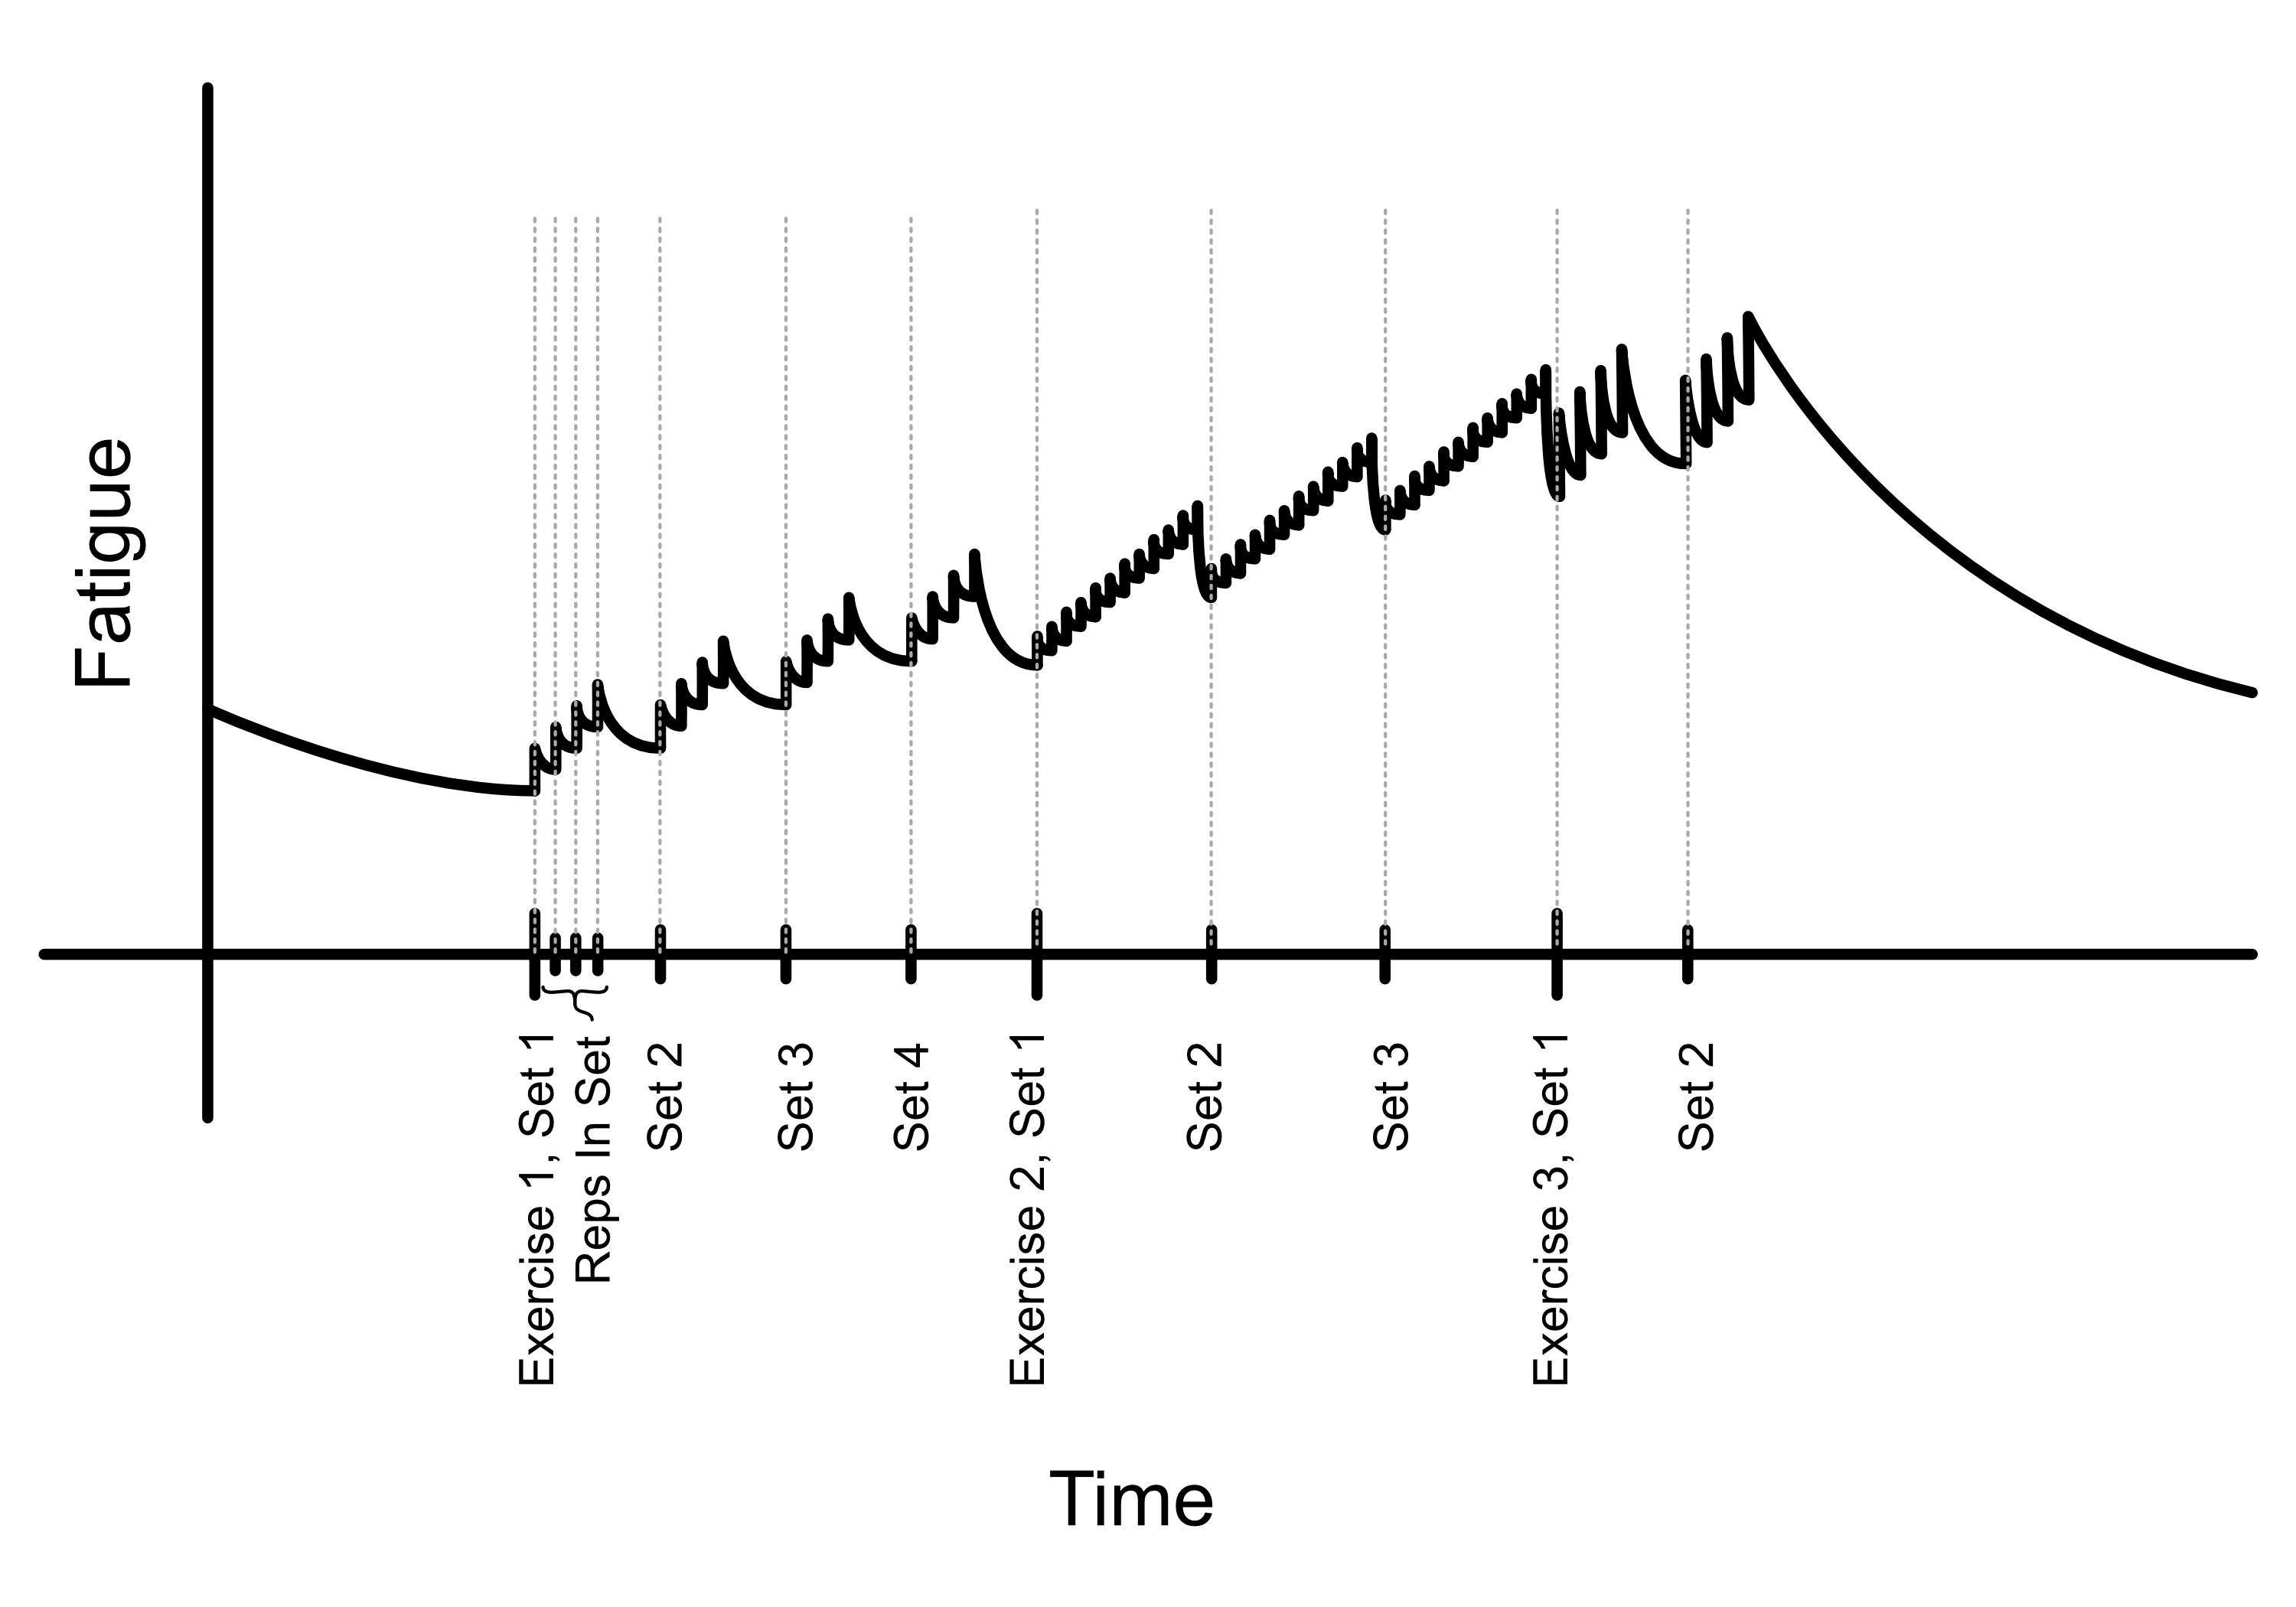
\includegraphics[scale=0.55]{images/p2/ch1/FatigueGraph.png}
    \caption{A graph that demonstrates how fatigue would respond over the course of a workout.}
    \label{fig:P2C1_GlobalFatigueGraph}
\end{figure}

The graph presented in figure \ref{fig:P2C1_GlobalFatigueGraph} has many things of interest. Probably the most important thing however is the time scale that fatigue is generated over. Looking at the graph, fatigue clearly has a very granular time scale that has precision on the order of magnitude with the time taken to complete each rep. There is no problem with this, but looking at the data described in chapter \ref{ch:DataSection} this granularity is not preserved. The data only has a date associated with it, making it only have a granularity of the scale of days. As shown in figure \ref{fig:P2C1_GlobalFatigueGraph} fatigue responds to changes several orders of magnitude smaller than a day. This will create huge problems later when trying to create any model. Ironically, the data itself will allow for an adaptation that fixes its own shortcoming. The key fact is that workouts are very standardized things. Reps are performed within sets, sets are performed within exercises, and exercises are performed within a workout. There are very distinct time scales associated with each part of the hierarchical structure. This hierarchical structure allows for fatigue to be tracked on separate time scales without explicitly knowing the time delta of each one and is what the fatigue categories presented in section \ref{sec:P1_ModifiedFatigueCategories} are derived from. 

\begin{figure}[htb]
    \centering
    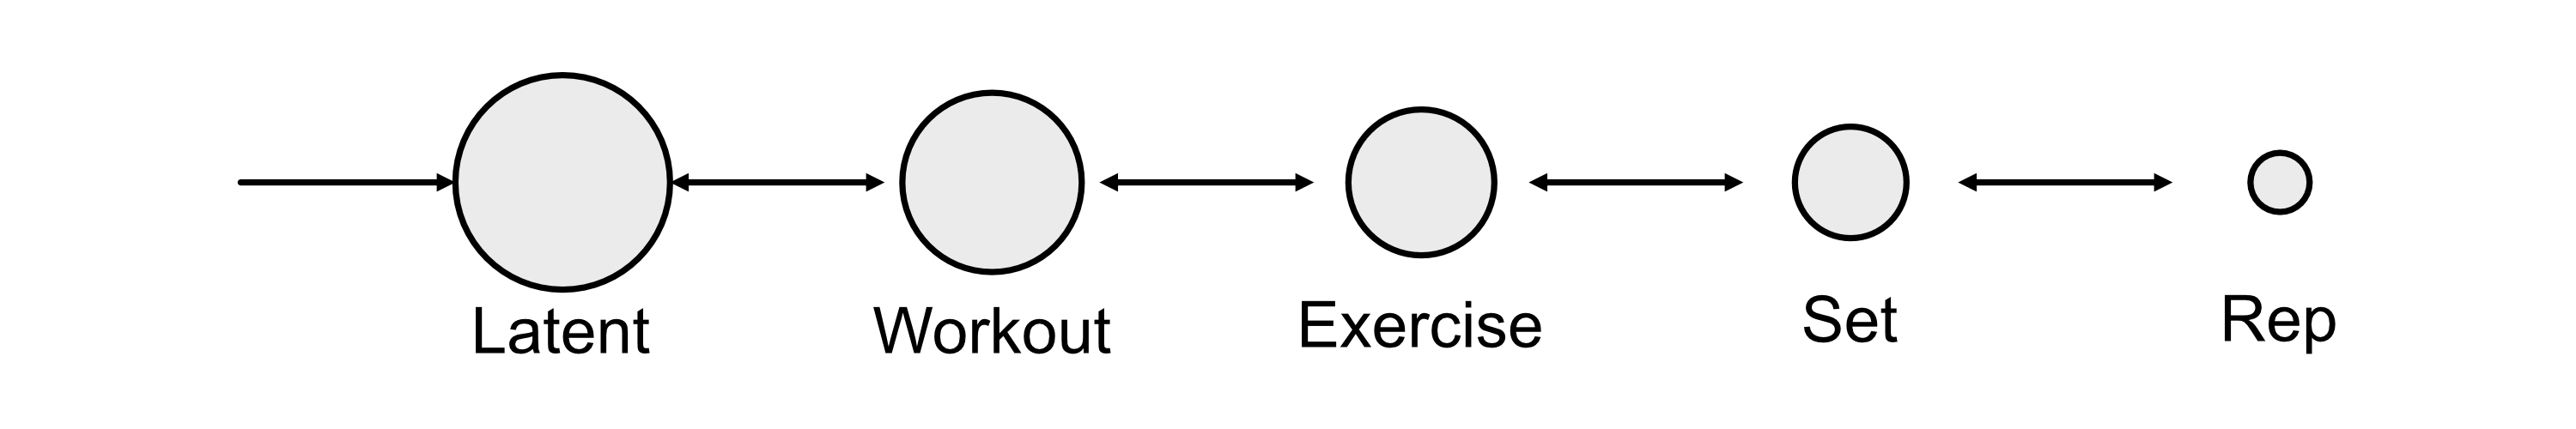
\includegraphics[scale=0.55]{images/p2/ch1/FatigueHierarchy.png}
    \caption{A figure that demonstrates fatigue hierarchy based on the different timescales it is comprised of.}
    \label{fig:P2C1_FatigueHierarchyGraph}
\end{figure}

As with anything that deals with time there is a "before" and a "after". For every level of this hierarchical structure there are a series of inputs and outputs that define what "before" and "after" is in regards to fatigue. This is why figure \ref{fig:P2C1_FatigueHierarchyGraph} has arrows that point in two directions. Generally, fatigue will be looked at before and after an action that produces fatigue is performed. Looking at figure \ref{fig:P2C1_GlobalFatigueGraph}, before every spike in fatigue there is a preexisting level of fatigue. This fatigue existed before the action was performed and needs to be taken into account because it affects the action that is about to be performed. After the spike there is a new higher level of fatigue, fatigue that now exists after the action was performed. Looking at fatigue this way not only enforces the summation of its parts to equal the total but it maintains fatigues state as actions are performed across time. Given this view, a more accurate representation of fatigue as it moves through time within the hierarchical structure is shown in figure \ref{fig:P2C1_FatigueHierarchyTimeGraph}.

\begin{figure}[htbp]
    \centering
    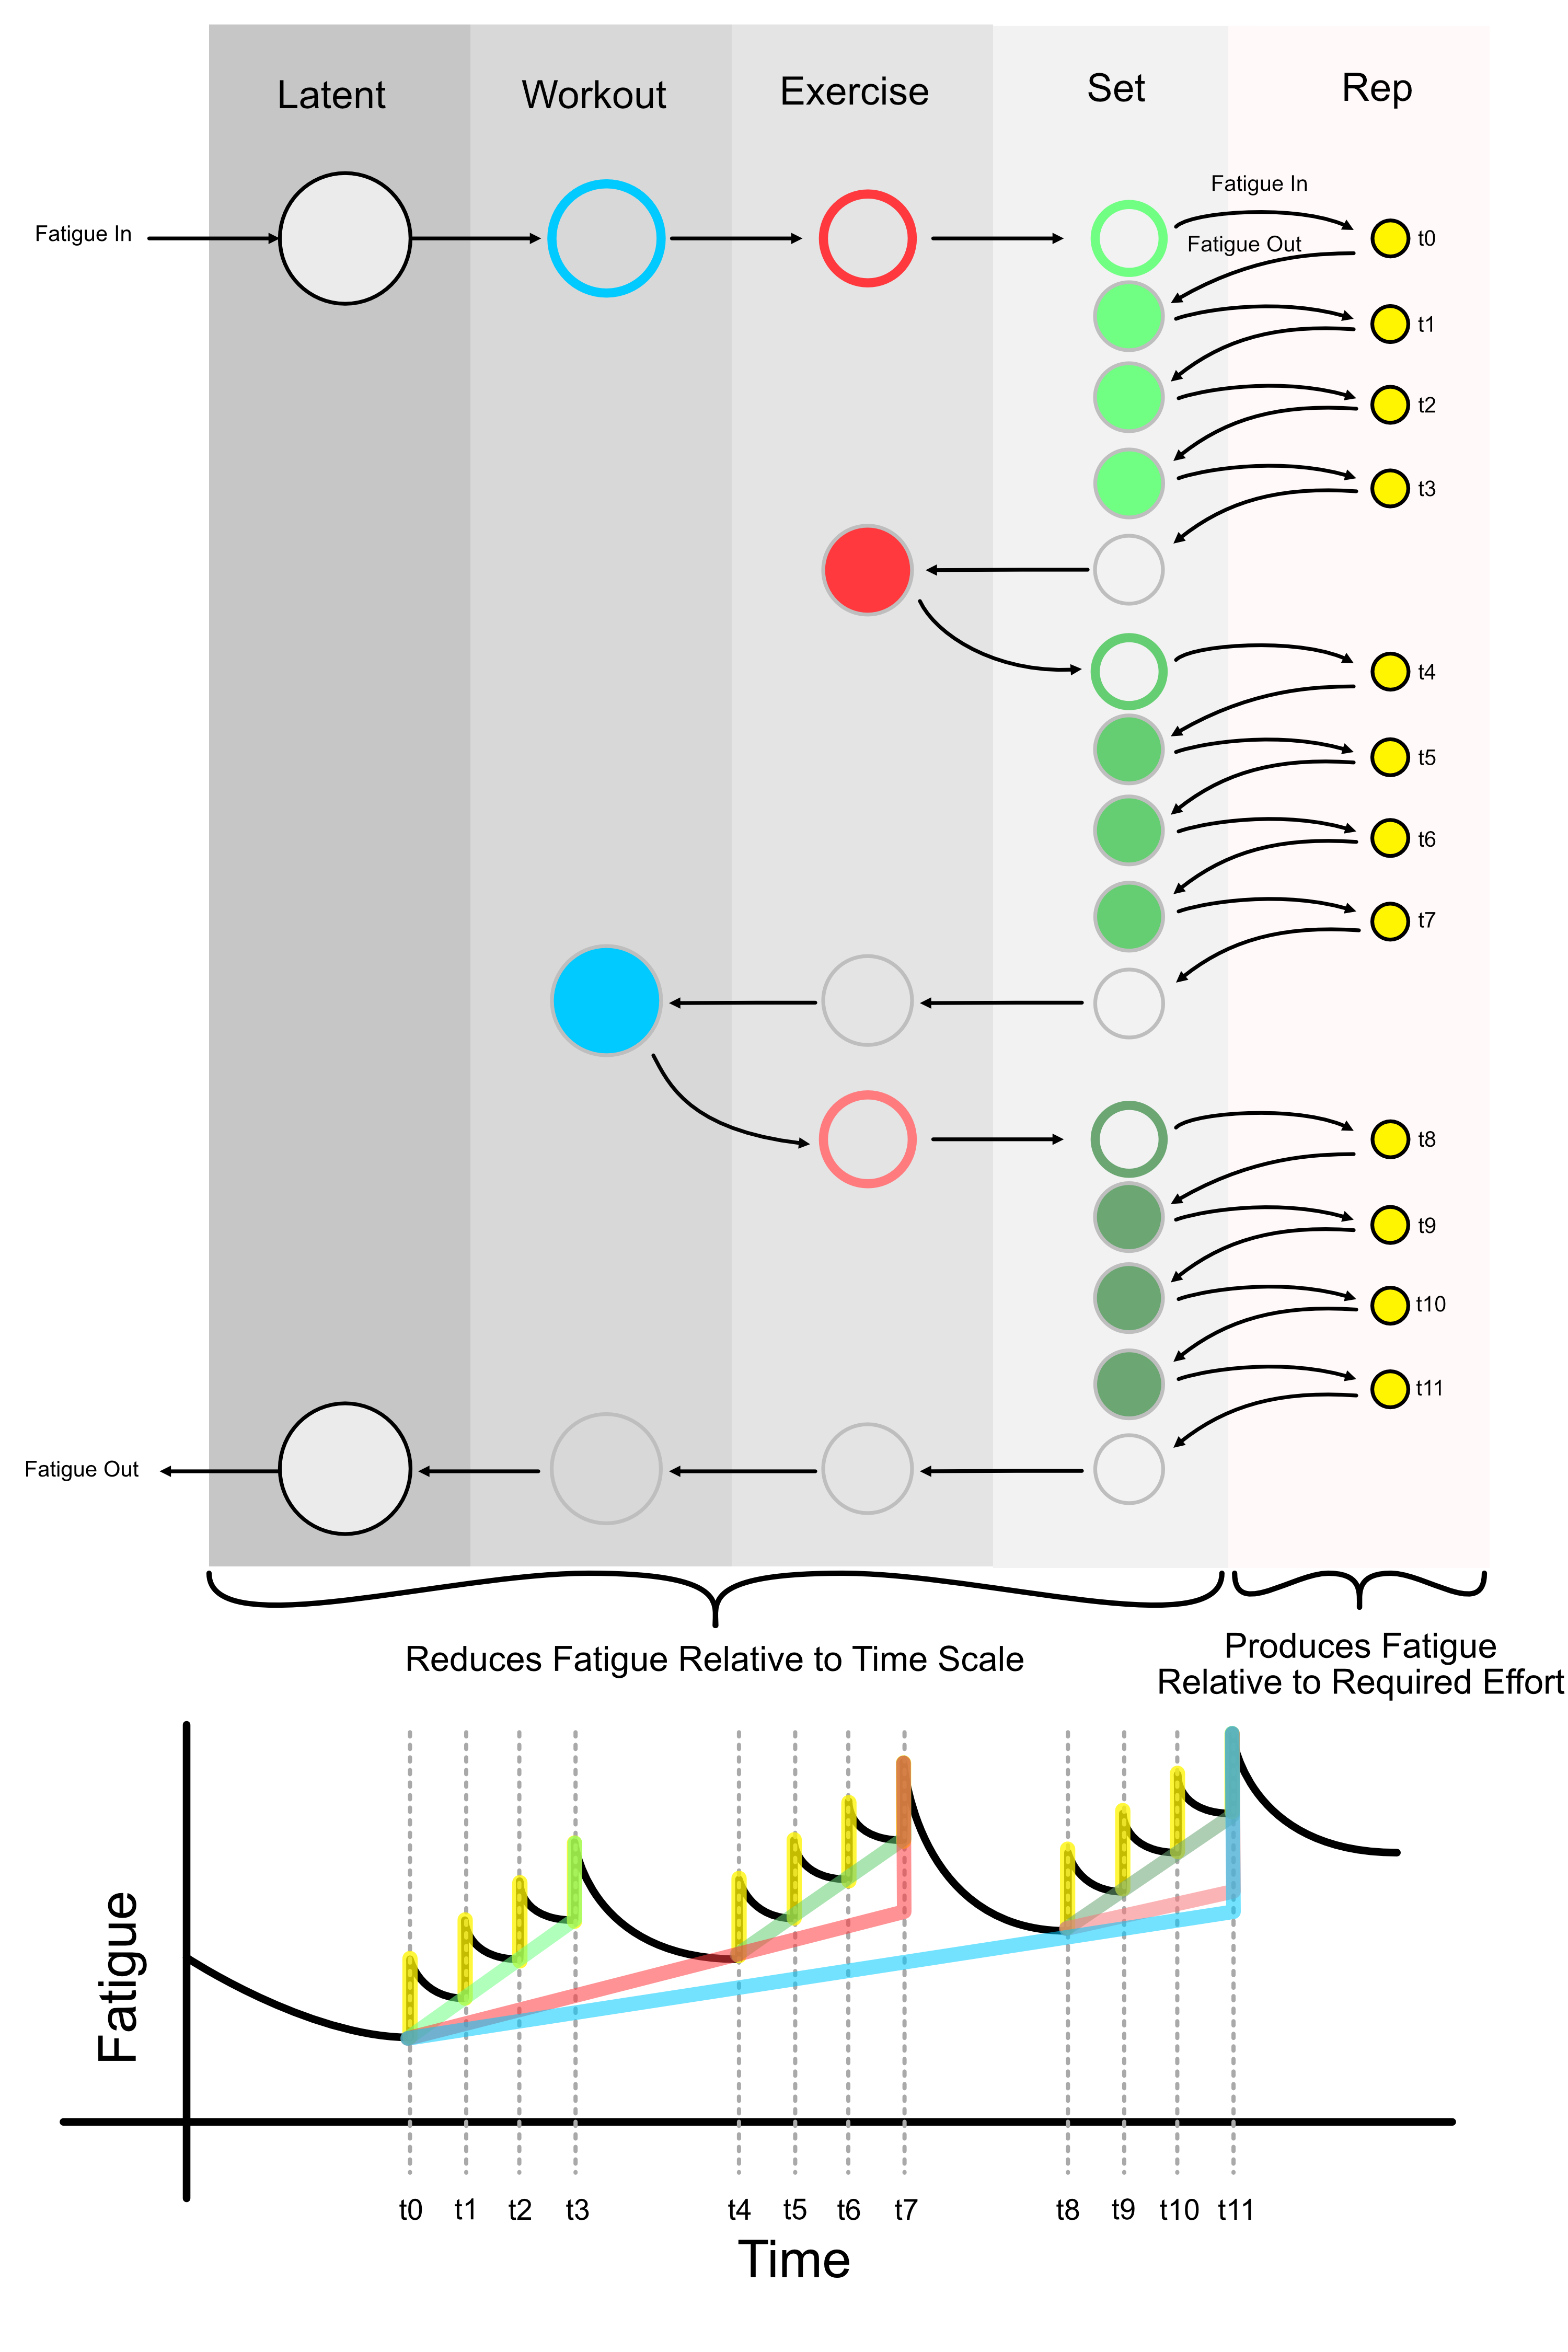
\includegraphics[scale=0.55]{images/p2/ch1/FatigueThroughTime.png}
    \caption{A figure that demonstrates the fatigues hierarchy as well as how fatigue moves through time through it. The graph on the bottom demonstrates where fatigue is measured.}
    \label{fig:P2C1_FatigueHierarchyTimeGraph}
\end{figure}

Figure \ref{fig:P2C1_FatigueHierarchyTimeGraph} has many important details. The first important detail is the action that each layer performs. The last layer, which demonstrates inter-rep fatigue, is the only layer to produce fatigue. All the other layers above it will act to reduce fatigue with a magnitude in correspondence to the time scale they represent. On a broader sense, every node, or circle, in the hierarchy has a transformation that it performs to fatigue such that the fatigue that it outputs is different from the input it receives. This is the mechanism that will create the multi-layered choppy look of the graph in figure \ref{fig:P2C1_GlobalFatigueGraph}. 

The second important detail is that not every node within the hierarchy will perform a transformation on fatigue. There will be nodes that simply exist as a 'pass through' to the appropriate layer which will apply the correct transformation. There are two groups of these pass through nodes. The first group will pass existing fatigue down to the next layer. This group is demonstrated in figure \ref{fig:P2C1_FatigueHierarchyTimeGraph} as hollow circles with colored borders. This represents the fatigue that is present before a rep is performed, or, as previously mentioned, the fatigue present "before" an action that generates fatigue.

The second group passes fatigue up the hierarchy. This occurs on boundaries where time scales end and a reduction in fatigue must be performed by the appropriate layer higher up in the hierarchy rather than the current layer. This group of nodes is represented by hollow circles with light grey borders in figure \ref{fig:P2C1_FatigueHierarchyTimeGraph}. The reasoning behind this group of nodes stems from recovery being a smooth, continuous process that does not occur discreet steps. Allowing every node in the hierarchy to reduce fatigue as timescales end and fatigue is propagated back up the hierarchy implies that there are discreet steps being applied. Instead, the highest node reached in the hierarchy should apply a single transformation that reduces fatigue to an appropriate level, matching the continuous nature of recovery. As an example, consider a scenario where a lifter finishes the last rep of the last set of an exercise. This will require the fatigue level from the last rep to be propagated through the inter-set, inter-exercise, and inter-workout layers. If every layer applied a transformation to fatigue it would be as if the lifter allowed inter-set fatigue to reduce before allowing inter-exercise fatigue to reduce and so on. This sequence of event does not happen, instead recovery is just happens at the largest time scale. To match this behavior the fatigue from the last rep is passed all the way up to the highest possible layer in the hierarchy, which for this example is inter-workout fatigue.

The adaptation of utilizing the time scale hierarchy has allowed for the model to capture many key nuances of fatigue on small timescales. This adaptation does not come for free however. The first limitation it imposes is requiring hierarchically structured data with respect to time scales. Any data that does not have this hierarchical structure to it will not fit within any model that is creating using this adaptation. For powerlifting this is not a problem but any sport that does not follow a structured plan will not fit within this model. The structure a sport imposes does not need to explicitly match the sets, reps, exercise, and workout structure that powerlifting uses. A sport may only employ the reps, exercise, and workout levels. This is ok, and is something that this model would in theory be able to understand with only minor tweaks. The true limitation of the model is when there is no structure whatsoever. If there is no structure then fatigue levels cannot be inferred at granular enough time scales to be useful. 

The second limitation stems from the model making assumptions about timescales within each layer. It is a well known fact that waiting longer before performing a physical task again will result in less fatigue being carried over to the next time the task is performed. If the time between each activity in the hierarchical model is not constant, for example the time between sets within a single exercise, then the model will have a very hard time accurately predicting fatigue. This is actually why breaking up fatigue into the discreet timescales presented in section \ref{sec:P1_ModifiedFatigueCategories} works. If this was not done then there would be no differentiation between the very different amounts of time spent resting between sets and reps and the relative changes in fatigue would not be captured. In laymans terms, the model assumes that the lifter takes breaks of constant length for each layer of the hierarchy.

%Given the discussion about how fatigue needs to move through time as well as the five different types of fatigue listed in section \ref{sec:P1_ModifiedFatigueCategories}, total fatigue can be represented with the equation below.
%
%\begin{equation}
%	\label{eq:P2C1_TotalFatigue}
%	F_{tot} \hat{=} F_l+F_w+F_e+F_s+F_r
%\end{equation}

With the general structure and limitations of fatigue having been talked about, the nuances of each time scale now need to be looked at.

\subsection{Inter-Rep Fatigue}
\label{sec:P2C1_InterRepFatigue}

Looking at figure \ref{fig:P2C1_GlobalFatigueGraph}, with every rep performed there is a spike in fatigue. The spike in fatigue is fairly self explanatory as performing a rep requires effort. A rep is the smallest time scale that needs to be recognized and as such every rep is considered to have taken zero time and will generate an impulse in fatigue. Looking at figure \ref{fig:P2C1_GlobalFatigueGraph} it should also be clear that different exercises will have different fatigue impulse magnitudes. The last exercise depicted in figure \ref{fig:P2C1_GlobalFatigueGraph} has a much greater impulse than the second exercise. This difference will require at least this part of the model to be fit to the data on a per exercise level. 

Something that figure \ref{fig:P2C1_GlobalFatigueGraph} does not do a good job communicating is that that fatigue impulse generated from a rep scales with the effort required to lift the weight. The idea behind this is reps that require extremely high effort will induce greater fatigue than reps that require less effort.

Given this discussion, the initial equation for $F_r$ is shown below. The $\epsilon_6$ term is a value that will be found after fitting the model to the data.

\begin{equation*}
	F_r=\epsilon_6 E
\end{equation*}

There is a problem with the equation shown above. When $F_r$ is considered in the context of the effort-fatigue model the $E_{tot}$ term already takes the form shown above.\footnote{This would be extremely bad for linear regression as this is the epitome of multicollinearity between $E_{tot}$ and $F_r$.} Given that $F_r$ takes the linear form shown above this says that any effort put into performing an exercise will be entirely spent on fatigue. This does not make sense because if that were the case then no sets above one rep could be performed as the effort put into that single rep would be entirely canceled out by the increase in fatigue and no effort would be left to power any further reps. The only time this scenario does make sense from the context of a 1RM. Given this insight, it is could be said that the effort term attached to $F_r$ needs to be sub-linearly scaled so that initially at low efforts many reps can be done but as effort approaches its maximum only a single rep can be done. Weather or not this sub-linear scaling is valid will need to be verified by the data. This approach is shown below in the final equation for $F_r$. Of note about the approach shown below is that the original case where effort is canceled out by the $F_r$ term can still be represented by having $\alpha=1$. When later chapters fit the model to data the magnitude of $|\alpha -1|$ will prove which approach is more accurate.

\begin{minipage}{\textwidth}
	\begin{equation}
		\label{eq:P2C1_InterRepFatigue}
		F_r=\epsilon_6 \left( \frac{E}{10} \right)^\alpha
	\end{equation}
	\centerline{where}
	\begin{equation*}
	    \alpha \ge 1
	\end{equation*}
\end{minipage}\\


\subsection{Inter-Set Fatigue}
\label{sec:P2C1_InterSetFatigue}

\begin{figure}[htb]
    \centering
    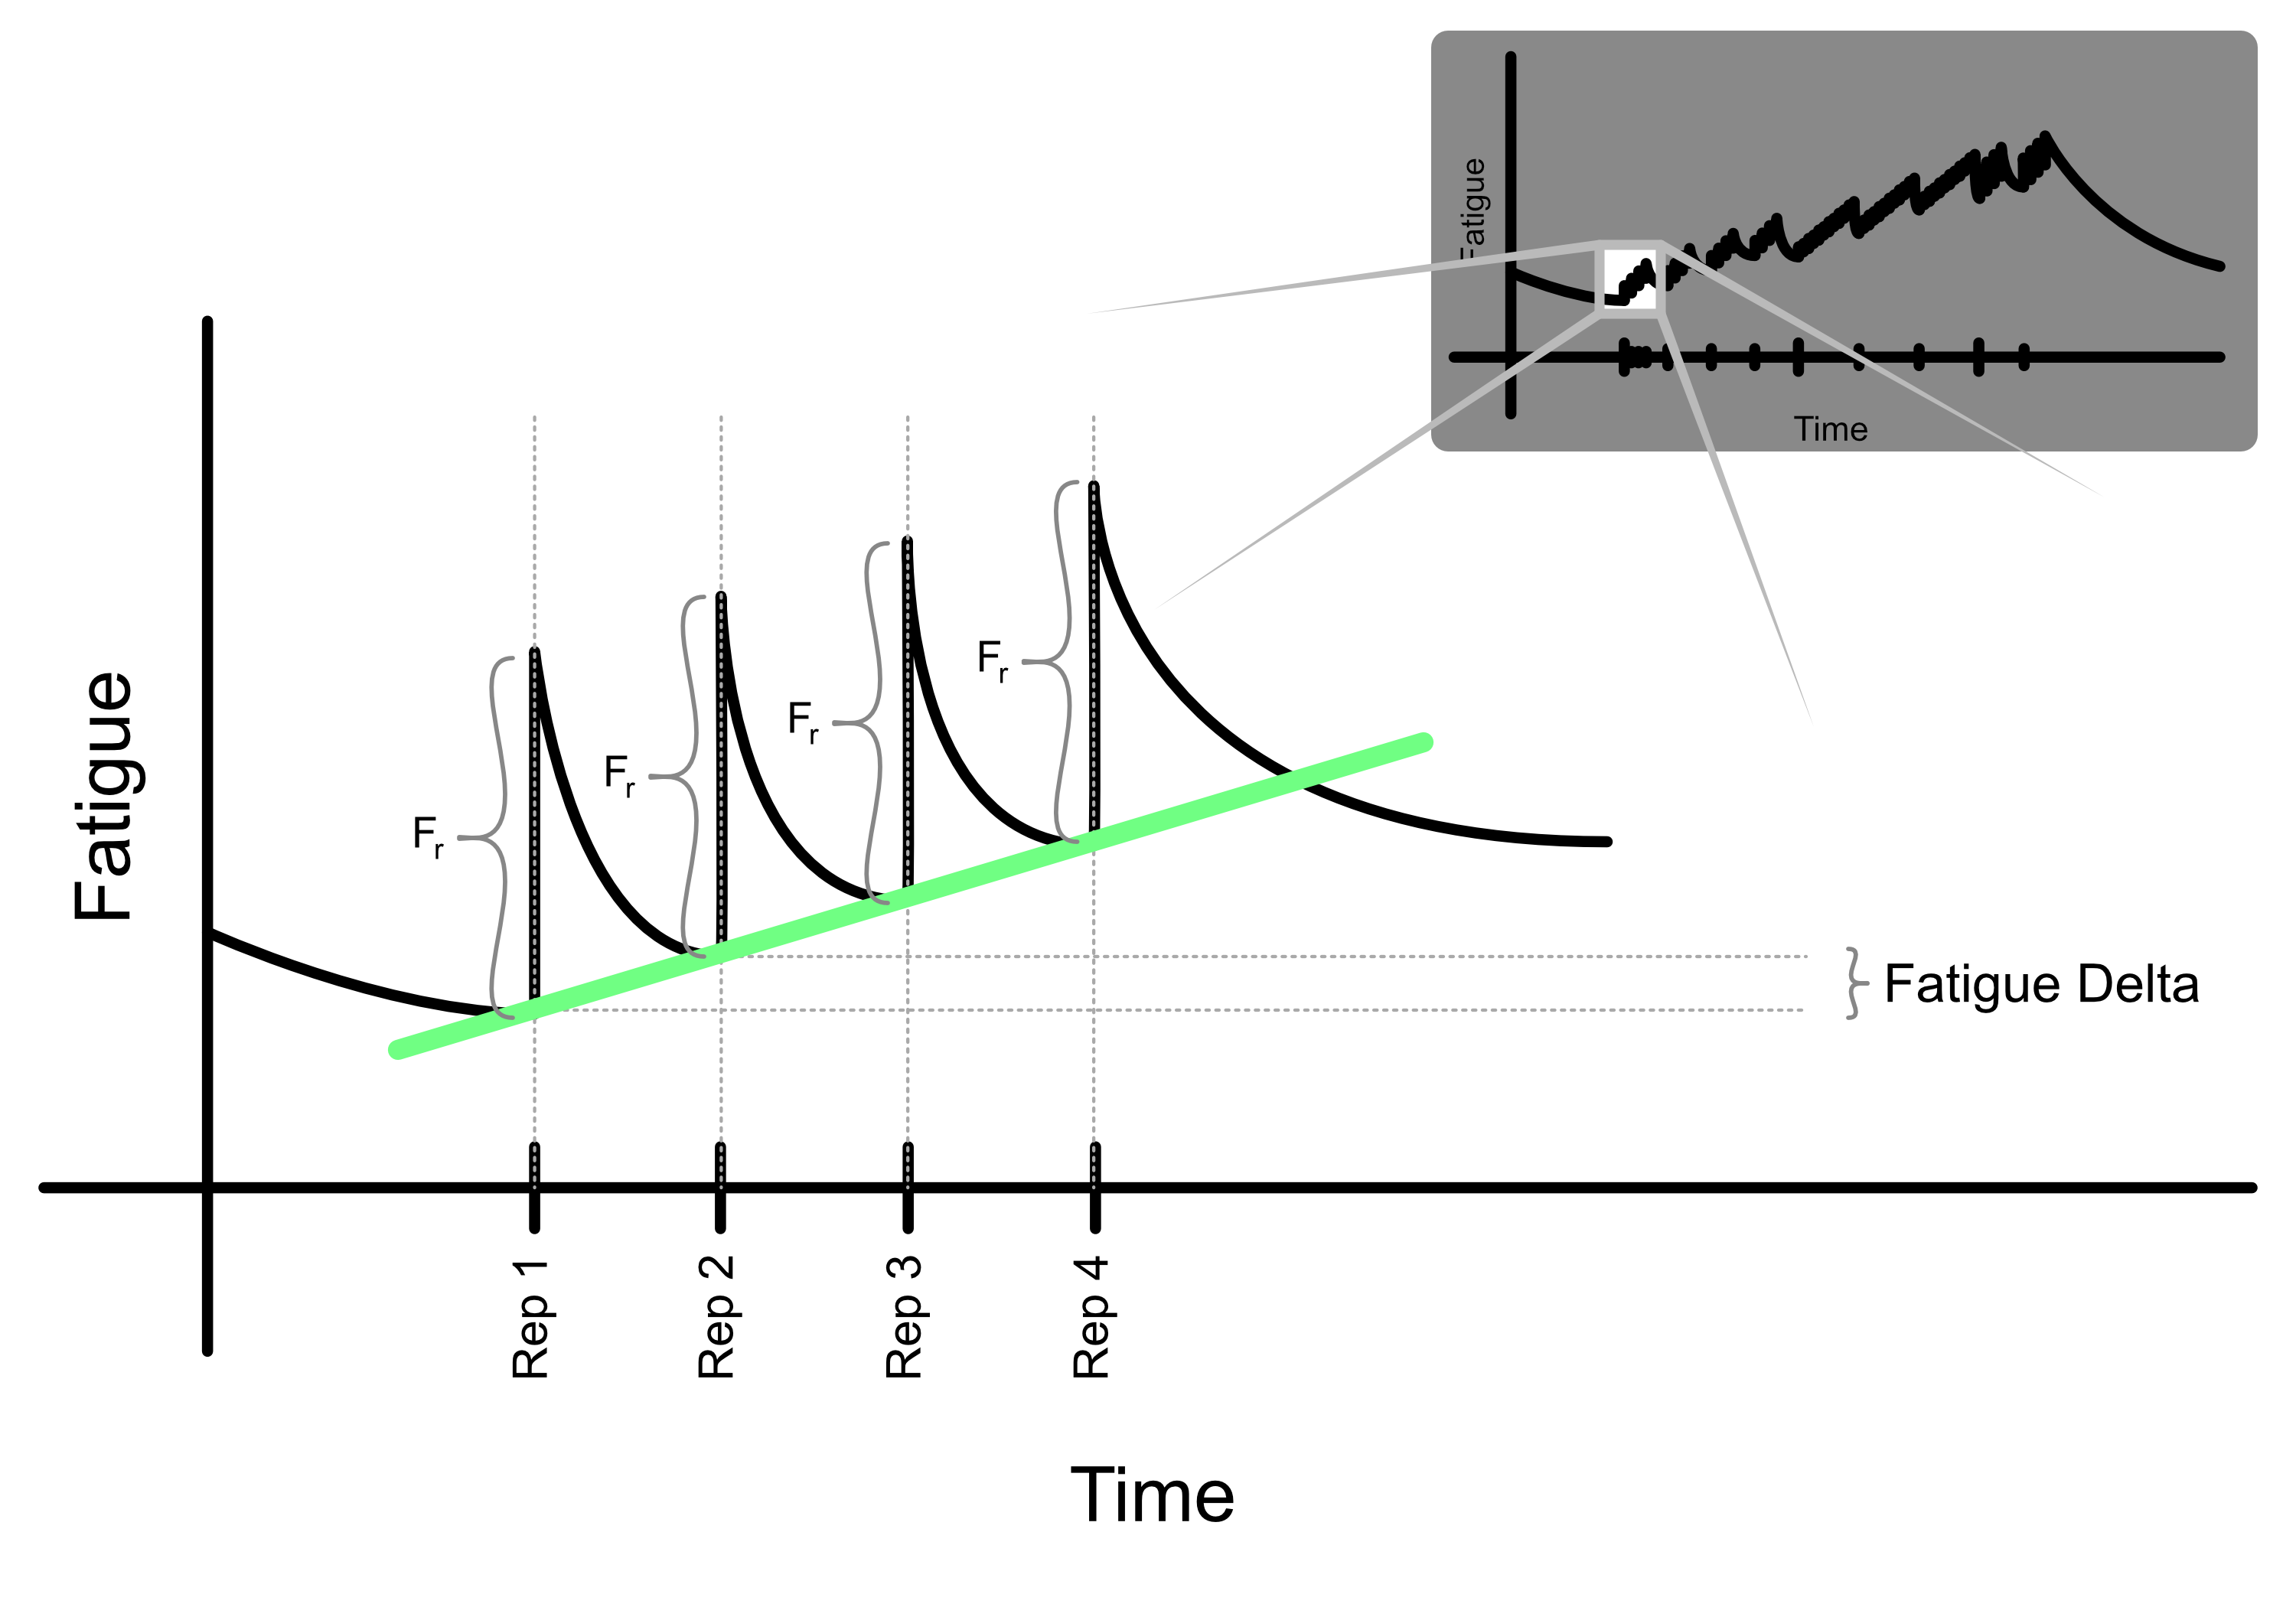
\includegraphics[scale=0.55]{images/p2/ch1/InterSetFatigue.png}
    \caption{A figure demonstrating how inter-set fatigue will accumulate over the course of a set from many fatigue impulses generated from performing reps.}
    \label{fig:P2C1_InterSetFatigue}
\end{figure}

Inter-set fatigue is composed of many inter-rep fatigue timescales. Figure \ref{fig:P2C1_InterSetFatigue} shows a section of figure \ref{fig:P2C1_GlobalFatigueGraph} zoomed in to focus on a single set. The green line that is superimposed on the graph depicts inter-set fatigue. In the graph there are impulses in fatigue generated from each rep which are then followed by slight reductions in fatigue. The slight reduction in fatigue is performed in the minuscule time between reps where a lifter is in a stable point that requires less energy expenditure than other points during the exercise. This small stable point is also where things like breathing can be safely performed which help reinvigorate the body and further reduce fatigue. The decrease in fatigue will never be able to match the impulse in fatigue generated by performing a rep which enforces a positive fatigue delta. If the body was able to decrease fatigue at a pace greater than or equal to the pace fatigue was generated then there would be a negative fatigue delta and a lifter would never have to stop exercising due to feeling tired. Outside of wishful thinking this is obviously not the case. Given that the fatigue delta will always be positive the important factor becomes the size of the delta. For endurance athletes, this delta needs to be as small as possible to allow for the smallest amount of accumulated fatigue as more and more reps are performed. Powerlifters rarely care about endurance, so minimizing the delta is not of major importance but the delta does still need to recognized as it will limit how many reps can be performed with a given weight.

Something implicitly stated in figure \ref{fig:P2C1_InterSetFatigue}, disregarding the spike at the end of the line, is inter-set fatigue increases linearly with the number of reps done. This does not necessarily need to be the case, and further analysis of the data will likely prove that the fatigue delta may not be a constant value and instead might increase as the number of reps increases which would imply that the body is recovering less and less from each impulse of fatigue. This distinction will require looking at the data, and will be one of the things discussed in the chapters to come.

From the previous section on inter-rep fatigue it is known that the magnitude of the fatigue impulse increases with the effort required to perform each rep. When this detail is considered in the context of inter-set fatigue something interesting happens. The time between reps remains relatively constant when compared to the magnitude of increase from the fatigue impulse. This means the body will have the same length of time to recover from a greater fatigue stimulus, which will lead to larger fatigue deltas, which will necessarily limit the number of reps performed with higher effort. This effect is shown in figure \ref{fig:P2C1_InterSetFatigueScaledByEffort} where the difference in fatigue delta is enough to make the total accrued fatigue from three reps performed at low effort to be less than that of two reps performed at high effort.

\begin{figure}[htb]
    \centering
    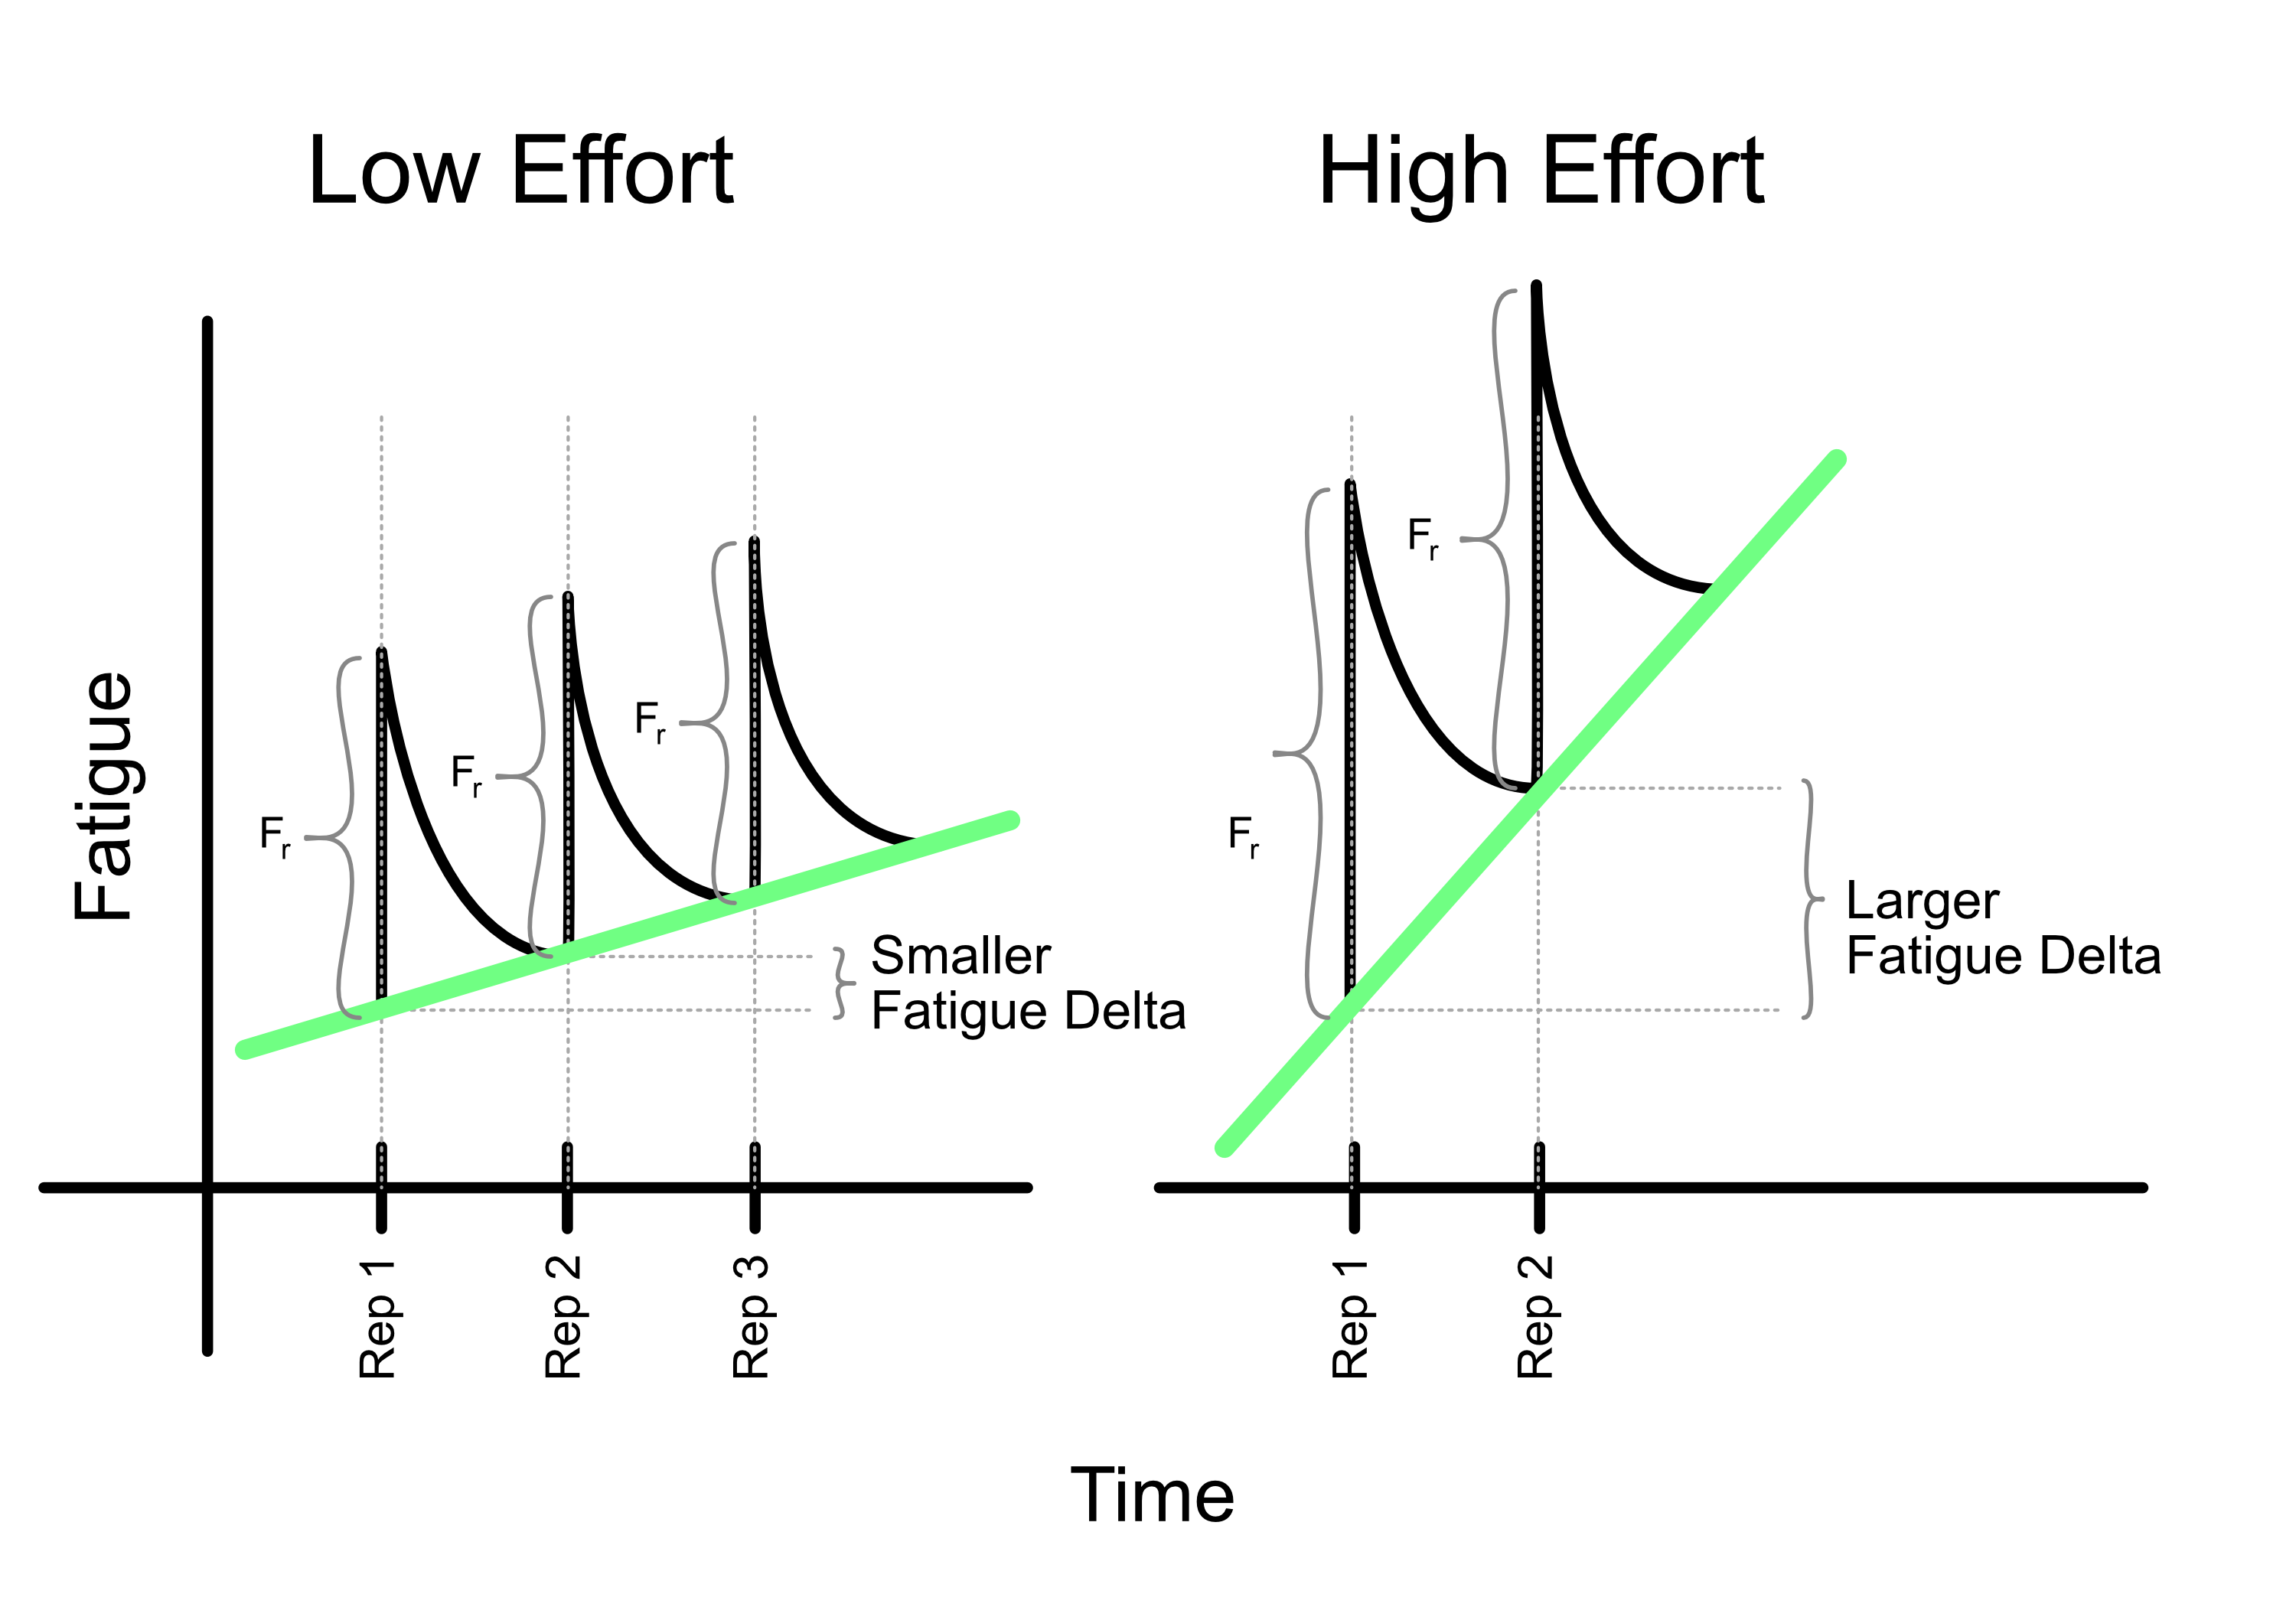
\includegraphics[scale=0.55]{images/p2/ch1/InterSetFatigueDeltaDifference.png}
    \caption{A figure demonstrating how differences in effort could affect the fatigue delta.}
    \label{fig:P2C1_InterSetFatigueScaledByEffort}
\end{figure}

The other notable feature about the green line in figure \ref{fig:P2C1_InterSetFatigue} is the spike at the end. This corresponds with the fatigue that is passed up the hierarchy as a timescale ends, which was discussed when talking about figure \ref{fig:P2C1_FatigueHierarchyTimeGraph}. As discussed previously, this is because inter-set fatigue does not apply the same reduction to the fatigue generated from the last rep as it does to the fatigue generated from every other rep. Instead, this fatigue is passed up the timescale hierarchy for the next layer which applies the correct transformation.

An equation needs to be generated given all of this discussion. An initial approach would be to sum up all the increases and decreases in fatigue to reach the final value. This is shown below.

\begin{minipage}{\textwidth}
	\begin{equation*}
		F_s=\sum_{i=1}^r F_r+\sum_{i=1}^{r-1} r_{rec,i}
	\end{equation*}
	\centerline{where}
	\begin{equation*}
		\begin{split}
			r_{rec,i} & \text{ represents the amount of recovery performed on rep }i \\
			|r_{rec,i}| & < 0
		\end{split}
	\end{equation*}
\end{minipage}\\

While this approach is correct it is not very efficient. To fix this the fact that adding the $i$th $F_r$ value to the $i$th $r_{rec,i}$ value will result in the $i$th fatigue delta will be used. Note that due to the bounds on the summations that there will be one $F_r$ term that does not have it's counterpart recovery term. This is done to match the behavior of the green line shown in figure \ref{fig:P2C1_InterSetFatigue}, specifically the spike at the end.

\begin{equation*}
	\begin{split}
		F_s & =
		\left( F_{r,1}+r_{rec,1} \right)+
		\left( F_{r,2}+r_{rec,2} \right)+
		\dots +
		\left( F_{r,r-2}+r_{rec,r-2} \right)+
		\left( F_{r,r-1}+r_{rec,r-1} \right)+
		F_{r,r}
		\\
		& = \Delta F_{r,1} +
		\Delta F_{r,2} +
		\dots +
		\Delta F_{r,r-2} +
		\Delta F_{r,r-1}+
		F_{r,r}
		\\
		& = F_{r,r}+\sum_{i=1}^{r-1}\Delta F_{r,i}
	\end{split}
\end{equation*}

This summation of fatigue deltas can now be represented as a single multiplication. To do this the $\Delta F_{r,i}$ terms will need to be constant, however, previously discussed in this section was the fact that these fatigue deltas may not be constant. This will need to be accounted for. To make it possible to transform this summation into a product every $\Delta F_{r,i}$ term will be scaled by some value, $c$, which will make the $\Delta F_{r,i}$ terms constant. 

\begin{equation*}
	F_s =
	F_{r} + \Delta F_r \sum_{i=1}^{r-1} c_i
\end{equation*}

This summation of $c_i$ values can now be represented as a function of $r$, $C(r)$.

\begin{equation*}
	F_s =
	F_{r} + \Delta F_r C(r)
\end{equation*}

Not much is really known about the behavior of this function as it depends entirely on how the fatigue deltas change as every additional rep is performed. The only thing that can be certain is that $c$ can only increase or stay the same as $i$ increases. If $c$ decreased then it would be as if the lifter were recovering \textit{more} with every additional rep performed, which cannot be the case. Put in mathematical terms, $C'(r)\ge0$. With this limited amount of information a function needs to be chosen that can allow for three scenarios to happen: the fatigue deltas increase at an increasing rate, stay the same, or increase at a decreasing rate. A power function can be used to approximate all of these scenarios and is shown in the equation below. Looking at the equation below, if $\beta=1$ then a constant fatigue delta is assumed, if $\beta>1$ then the fatigue deltas increase at an increasing rate, and if $0<\beta<1$ then the fatigue deltas increase at a decreasing rate. $\beta$ must be constrained to being $>0$ otherwise $C'(r)$ would be $<0$. Depending on the value of $\beta$ that is found from fitting the model to the data it will be able to show how the body responds to fatigue on a inter-set level.

\begin{equation*}
	F_s =
	F_{r} + (r-1)^\beta \Delta F_r
\end{equation*}

The last missing piece is how to represent $\Delta F_r$ as it is not something that is directly available. Given that it is a constant it can simply be represented as a fraction of the total $F_r$ value. To do this a $\epsilon_5$ term will be added and it will be restricted to the domain of $0 \le \epsilon_5 \le 1$. Once the model is fit to the data the value of $\epsilon_5 (r-1)^\beta$ will be able to show how much recovery is performed on a given rep within the context of a set.

\begin{equation*}
	F_s =
	F_{r} + \epsilon_5 (r-1)^\beta F_r
\end{equation*}

After a little help from intuition, equation \ref{eq:P2C1_InterSetFatigue} is the final equation that represents inter-set fatigue.

\begin{minipage}{\textwidth}
	\begin{equation}
		\label{eq:P2C1_InterSetFatigue}
		\begin{split}
			F_s & = \epsilon_5 (r-1) ^ \beta F_r + F_r
			= \epsilon_5 \epsilon_6 (r-1)^\beta \left( 
				\frac{E}{10} 
			\right)^\alpha
			+ \epsilon_6 \left( \frac{E}{10} \right)^\alpha
			\\
			& = 
			\epsilon_6 \left( \frac{E}{10} \right)^\alpha
			\left(
				\epsilon_5 (r-1)^\beta + 1
			\right)
		\end{split}
	\end{equation}
	\centerline{where}
	\begin{equation*}
		\begin{split}
		    & \alpha \ge 1 \\
		    & \beta > 0 \\
			& 0 \le \epsilon_5 \le 1
		\end{split}
	\end{equation*}
\end{minipage}\\

\subsection{Inter-Exercise Fatigue}
\label{sec:P2C1_InterExerciseFatigue}

\begin{figure}[htb]
    \centering
    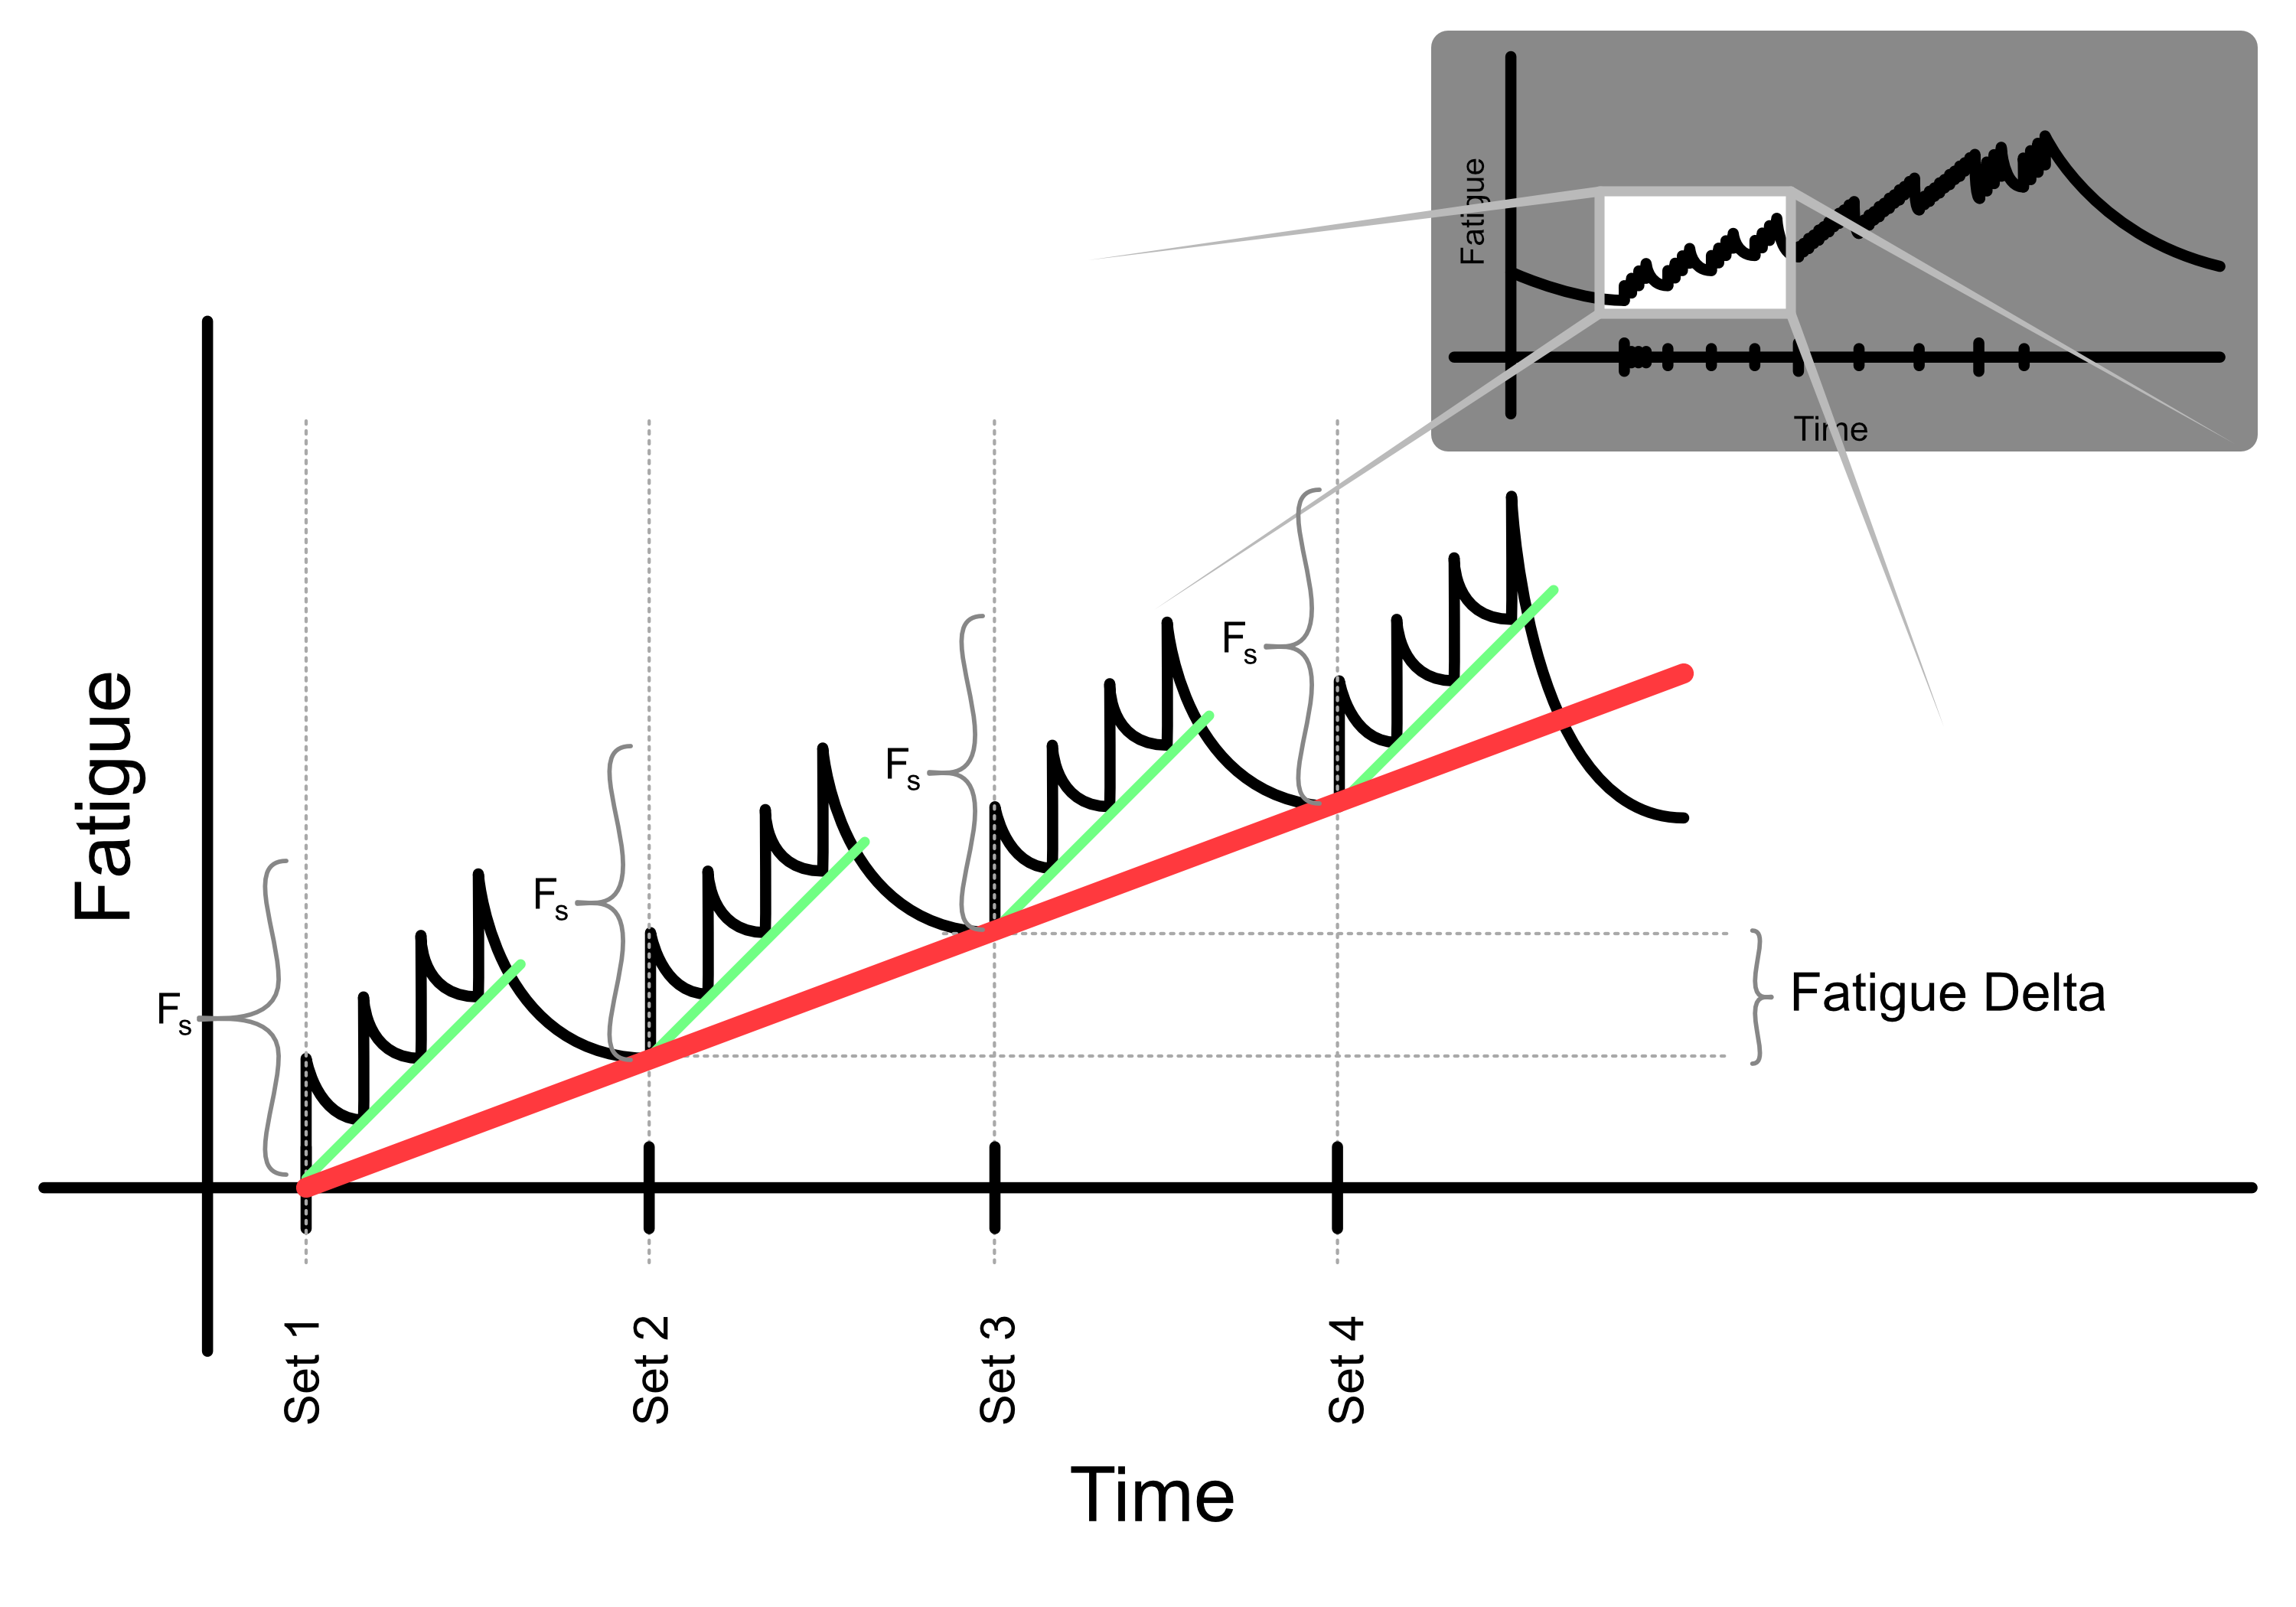
\includegraphics[scale=0.55]{images/p2/ch1/InterExerciseFatigue.png}
    \caption{A figure demonstrating how inter-exercise fatigue will accumulate over the course of several sets.}
    \label{fig:P2C1_InterExerciseFatigue}
\end{figure}

Inter-exercise fatigue is very similar to inter-set fatigue except  it operates one level higher in the timescale hierarchy. This is demonstrated in figure \ref{fig:P2C1_InterExerciseFatigue} where the superimposed red line is inter-exercise fatigue. The red line in figure \ref{fig:P2C1_InterExerciseFatigue} combines many inter-set fatigue lines which are shown in green. Of note is that inter-exercise fatigue shares the same behavior with the spike at the end of the red line. This is for the same reason as inter-set fatigue, just now it is one level up the timescale hierarchy.

Given the extreme parallels between inter-set fatigue and inter-exercise fatigue, the resulting equation for inter-exercise fatigue can simply be stated.

\begin{minipage}{\textwidth}
	\begin{equation}
		\label{eq:P2C1_InterExerciseFatigue}
		\begin{split}
			F_e & = \epsilon_4 (s-1) ^ \gamma F_s + F_s \\
				& = F_s\left( \epsilon_4 (s-1)^\gamma+1  \right) \\
				& = 	\epsilon_6 \left( \frac{E}{10} \right)^\alpha
					\left( \epsilon_5 (r-1)^\beta + 1 \right)
					\left(\epsilon_4 (s-1)^\gamma+1  \right)
		\end{split}
	\end{equation}
	\centerline{where}
	\begin{equation*}
		\begin{split}
		    & \alpha \ge 1 \\
		    & \beta,\gamma > 0 \\
			& 0 \le \epsilon_4, \epsilon_5, \epsilon_6 \le 1
		\end{split}
	\end{equation*}
\end{minipage}\\


\subsection{Inter-Workout Fatigue}
\label{sec:P2C1_InterWorkoutFatigue}

\begin{figure}[htb]
    \centering
    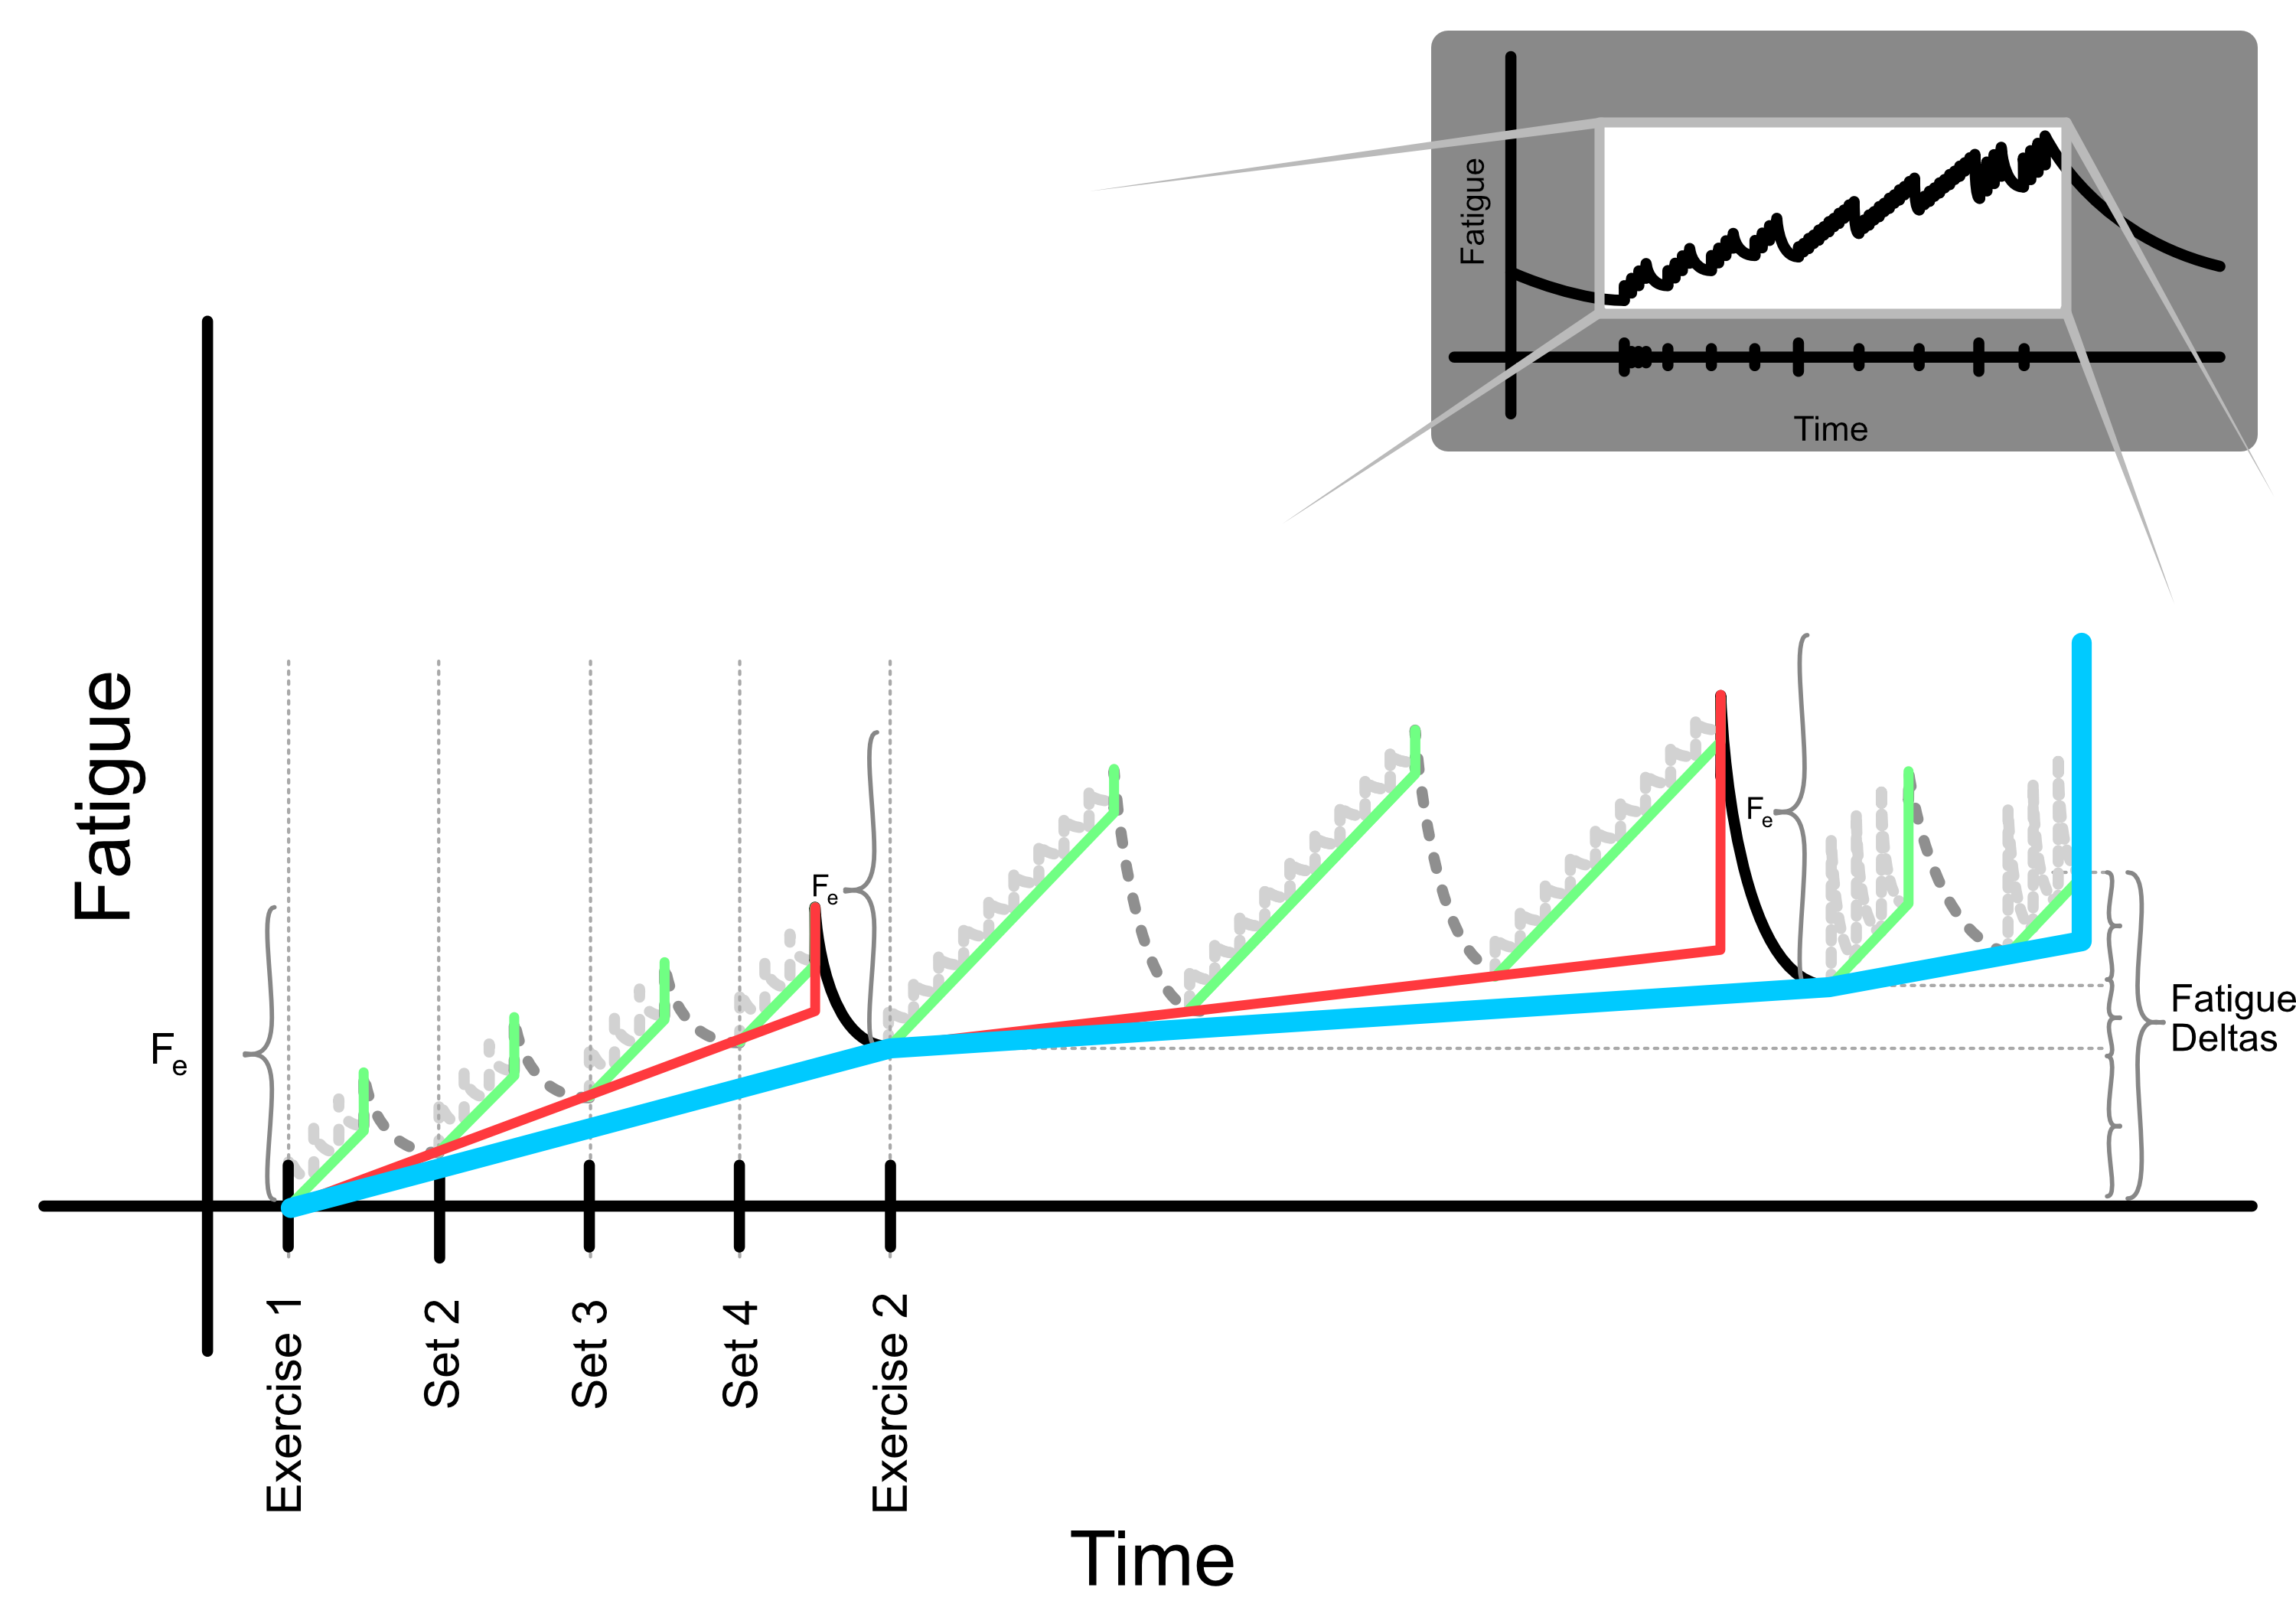
\includegraphics[scale=0.55]{images/p2/ch1/InterWorkoutFatigue.png}
    \caption{A figure demonstrating how inter-workout fatigue will accumulate over the course of several exercises.}
    \label{fig:P2C1_InterWorkoutFatigue}
\end{figure}

Given the terse nature of the section about inter-exercise fatigue it may seem like this section will be the same. There is a pattern present and for the most part this pattern will continue but on this scale there are more variables to think about. The previous sections on inter-workout fatigue and inter-set fatigue had the luxury of being able to use the same values for reps, sets, and effort. The timescales at those levels of the fatigue hierarchy were small enough to allow each of them to only need to rely on a single data point. This certainly made it easier to discover relations, but it is not a luxury that inter-workout fatigue can depend on. Inter-workout fatigue will need to look at many data points that span the length of an entire workout. Having a mechanism like this that considers many data points is the first feedback mechanism that is present in the model. This is important because this is how the model will take into account previous perturbations in fatigue.

Figure \ref{fig:P2C1_InterWorkoutFatigue} shows a zoomed in section of \ref{fig:P2C1_GlobalFatigueGraph}. Superimposed are green lines that represent inter-set fatigue, red lines to represent inter-exercise fatigue, and a blue line to show inter-workout fatigue. The behavior between the red line and green line is very different from the behavior between the blue line and red line. The non-continuous nature of the blue line is the defining difference that needs to be discussed.

The non-continuous nature of inter-workout fatigue can be traced back to the red lines not forming a clear pattern that the blue line can extrapolate. The reason for this lack of a pattern is because inter-workout fatigue needs to take into consideration fatigue carried over between exercises that use similar muscle groups as well as differing effort levels between exercises. As an example, consider that when a lifter switches exercises fatigue drops depending on the amount of similarity between the exercises. If two exercises are similar more fatigue will carry over between them, increasing the perceived inter-workout fatigue and by extension fatigue on any level in the fatigue hierarchy lower than inter-workout fatigue. On some occasions this is purposeful, and is used as a way to increase stimulus while keeping intensity low. As another example, consider that every exercise has differing effort levels. As previously established in the inter-set and inter-rep fatigue sections fatigue will increase with increased effort. If the same exercise is performed twice with differing effort levels then the fatigue delta on the inter-workout scale will be different for each one because they caused different increases in fatigue. These relative differences in fatigue levels based on what exercises were performed previously as well as what effort they were performed at is what makes inter-workout fatigue non-continuous. 

The discussion about ordering of exercises brings up a more general idea of the time delta between similar exercises. Lets say two exercises that are very similar to each other are performed in the same workout. If these exercises are performed back to back then the second exercise will have a much higher level of fatigue than if they were performed at the beginning and end of the same workout respectively. This difference in fatigue levels happens despite the exercises being identical in terms of sets, reps, intensity, and effort. The only difference is the amount of time that passed between performing the two exercises. If the exercises are performed back to back then there will be very little time to recover and as such not as much recovery will be done. If instead they are performed at the beginning and end of a workout then the lifter would have had the entire length of the workout for those muscle groups to recover. This can be generalized to simply state that fatigue carryover between exercises will increase the closer in time two exercises are.

To further clarify with a more concrete example, if a lifter begins their workout with squats, their lower body will be more fatigued than their upper body. If the same lifter then changes exercises to bench, they will be less fatigued for an upper body exercise than they would be for another lower body exercise, although, they will still be more fatigued than if they started their workout with bench. This example is further demonstrated in figure \ref{fig:P2C1_InterWorkoutExerciseOrder}. In figure \ref{fig:P2C1_InterWorkoutExerciseOrder} exercise 1 would be squats from the example. Exercise 2 is another another lower body exercise and exercise 3 is an upper body exercise. The graph on the left in figure \ref{fig:P2C1_InterWorkoutExerciseOrder} shows exercise 2 being performed right after exercise 1, and the graph on the right places exercise 3 before exercise 2. Note how the inter-workout fatigue performed between exercise 1 and 2 on the left graph is small, which results in higher fatigue levels for the entirety of exercise 2. On the right graph the larger time difference between exercise 1 and 2 allows for more recovery to be performed, reducing fatigue levels. Another observation is that inter-workout fatigue is consistently less in the right graph because the ordering of the exercises maximizes the amount of recovery that can be performed. \footnote{Epic foreshadowing...}

\begin{figure}[htb]
    \centering
    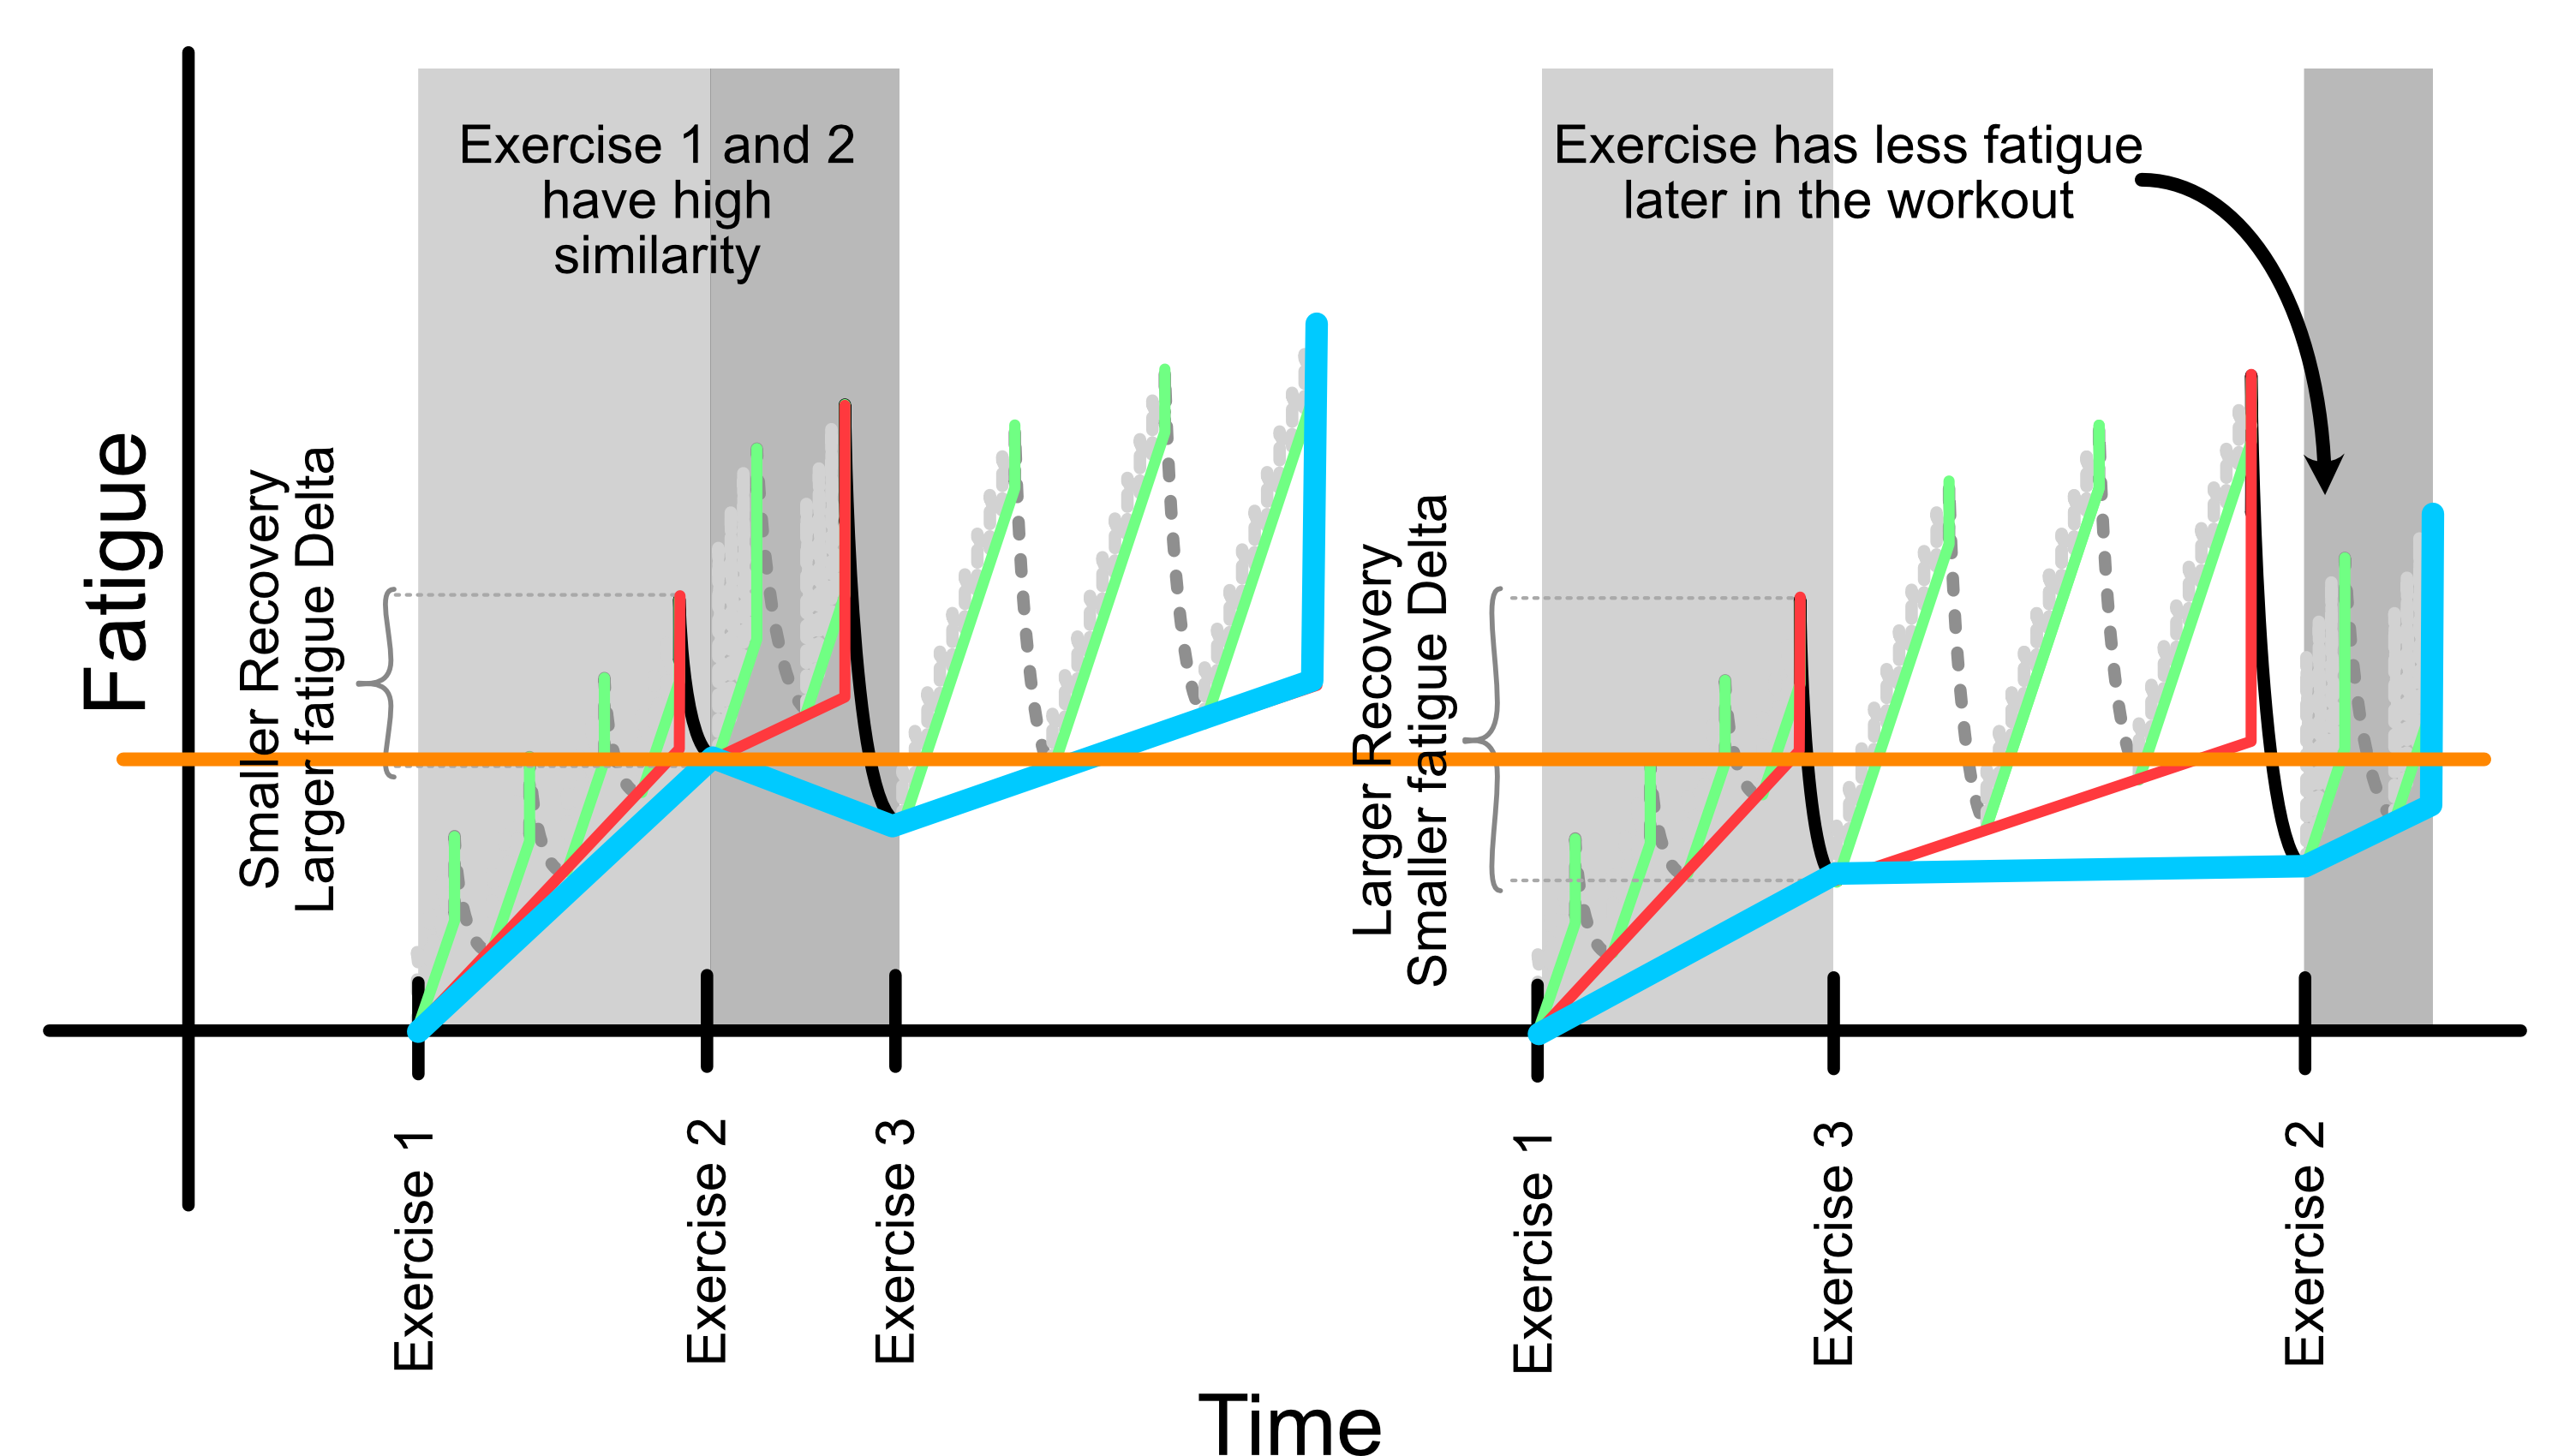
\includegraphics[scale=0.55]{images/p2/ch1/InterWorkoutExerciseOrder.png}
    \caption{A figure demonstrating how inter-workout fatigue will vary depending on the ordering of exercises within a workout.}
    \label{fig:P2C1_InterWorkoutExerciseOrder}
\end{figure}



All the feedback present in inter-workout fatigue makes it difficult to express. As a starting point, the simplest way to represent inter-workout fatigue is through a summation of the changes to fatigue on the level of inter-exercise fatigue.

\begin{minipage}{\textwidth}
	\begin{equation*}
		F_w=\sum_{i=1}^{n_e} F_e+\sum_{i=1}^{n_e-1} e_{rec,i}
	\end{equation*}
	\centerline{where}
	\begin{equation*}
		\begin{split}
			n_e & \text{ represents the total number of exercises performed in a workout} \\
			e_{rec,i} & \text{ represents the amount of recovery performed after exercise }i \\
			|e_{rec,i}| & < 0 \\
		\end{split}
	\end{equation*}
\end{minipage}\\

The same simplifications that were applied in the section about inter-set fatigue can be applied here up to a point, resulting in the equation below.

\begin{equation*}
	F_w =
	F_{e} + \epsilon_3 F_e \sum_{i=0}^{n_e-1} c_i
\end{equation*}

At this point the relative differences in recovery caused by the feedback present in inter-workout fatigue need to be considered. The previous sections on inter-exercise and inter-set fatigue reached this point and they were able to find a consistent pattern with the recovery performed that enabled the removal of the summation. This section cannot rely on this behavior, so to proceed the nature of each $c_i$ term needs to be considered. 

The first component of each $c_i$ term comes from effort. The fatigue delta from a given exercise will increase with the number of reps performed and the level of effort those reps required. As discussed previously fatigue may not scale linearly with effort. For this reason the effort term will be raised to a power, $\mu$. This looks very similar to the equation from inter-rep fatigue, but they are separate values. This summation is not calculating the total fatigue by summing up every exercises inter-rep fatigue. It is calculating the fatigue delta, which will increase with increases in inter-rep fatigue but is not equal to inter-rep fatigue. This distinction is important because it separates the inter-rep fatigue term from the effort term in this equation even though they have similar behaviors. The fatigue delta should increase with increases in effort, which constrains $\mu$ to being $>0$. If $\mu>1$ then there will be increasing returns in the fatigue delta from increasing effort levels. If $\mu=1$ then there will be constant increases in the fatigue delta, and if $0<\mu<1$ then there will be decreasing returns to the fatigue delta as effort increases. The value of $\mu$ will be found by fitting the model to the data.

The second component of each $c_i$ term comes from the similarity between exercises with respect to time. The fatigue delta will increase with greater similarity between exercises that were previously performed, represented by $S(i,j)$. This $S(i,j)$ term is then scaled by time such that exercises performed earlier in the workout end up reducing the fatigue delta. The behavior of the fatigue delta relative to time is not exactly known. Similar to the effort term, a constant, $\eta$, will be added to allow the model to understand different behaviors. The ranges of $\eta$ that have differing behaviors are the same as $\mu$.

\begin{minipage}{\textwidth}
	\begin{equation*}
		c_i=s_i r_i E_i^\mu \sum_{j=0}^{j=i-1} S(i,j)(n_e-j)^\eta
	\end{equation*}
	\centerline{where}
	\begin{equation*}
		\begin{split}
			& S(i,j) \text{ represents a similarity score between exercise }i \text{ and exercise }j \\
			& \mu, \eta>0
		\end{split}
	\end{equation*}
\end{minipage}\\

This equation for $c_i$ can be placed in the equation for $F_w$.

\begin{minipage}{\textwidth}
	\begin{equation*}
		F_w =
			F_{e} + 
			\epsilon_3 F_e 
			\sum_{i=0}^{n_e-1} \left( 
				s_i r_i E_i^\mu 
				\sum_{j=0}^{j=i-1} S(i,j)(n_e-j)^\eta
			\right)
	\end{equation*}
	\centerline{where}
	\begin{equation*}
		\begin{split}
			& n_e \text{ represents the total number of exercises performed in a workout} \\
			& S(i,j) \text{ represents a similarity score between exercise }i \text{ and exercise }j \\
			& \mu, \eta>0
		\end{split}
	\end{equation*}
\end{minipage}\\

With all of that, the final equation for inter-workout fatigue is shown in equation \ref{eq:P2C1_InterWorkoutFatigue}.

\begin{minipage}{\textwidth}
	\begin{equation}
		\label{eq:P2C1_InterWorkoutFatigue}
		\begin{split}
			F_e & = 
			\epsilon_3 F_e 
			\sum_{i=0}^{n_e-1} \left( 
				s_i r_i E_i^\mu 
				\sum_{j=0}^{j=i-1} S(i,j)(n_e-j)^\eta
			\right)
			+ F_e \\
			& = F_e \left(
				\sum_{i=0}^{n_e-1} \left( 
					s_i r_i E_i^\mu 
					\sum_{j=0}^{j=i-1} S(i,j)(n_e-j)^\eta
				\right)
			\right)
			\\
			& = \epsilon_6 \left( \frac{E}{10} \right)^\alpha
				\left( \epsilon_5 (r-1)^\beta + 1 \right)
				\left(\epsilon_4 (s-1)^\gamma+1  \right)
				\left(
					1+\epsilon_3 \sum_{i=0}^{n_e-1} \left( 
						s_i r_i E_i^\mu 
						\sum_{j=0}^{j=i-1} S(i,j)(n_e-j)^\eta
					\right)
				\right)
			\\
		\end{split}
	\end{equation}
	\centerline{where}
	\begin{equation*}
		\begin{split}
		    & \alpha \ge 1 \\
		    & \beta,\gamma, \mu, \eta > 0 \\
			& 0 \le \epsilon_3, \epsilon_4, \epsilon_5, \epsilon_6 \le 1 \\
			& n_e \text{ represents the total number of exercises performed in a workout} \\
			& S(i,j) \text{ represents a similarity score between exercise }i \text{ and exercise }j \\
		\end{split}
	\end{equation*}
\end{minipage}\\

\subsection{Latent Fatigue}
\label{sec:P2C1_LatentFatigue}

The last fatigue category is latent fatigue. This category has the largest timescale and is responsible for capturing fatigue between workouts. The large timescale of latent fatigue makes it very difficult to fully capture. Many factors that exist outside of the gym can increase a lifters stress which will affect latent fatigue. Things like a lack of sleep, poor diet, stress at work or from a relationship, and many other things can create stress that will increase latent fatigue and limit performance at the gym. These factors are largely invisible to the model as there is simply no data that can capture these nuances. Instead, these nuances will simply be seen by the model as consistent deltas from what it predicts. These deltas will need to be accounted for in order for the model to perform accurately, and is where the model will need to adapt to the user. \footnote{Even more epic foreshadowing...} In order for the model to properly adapt the latent fatigue that is generated from workouts will need to be accounted for, which will allow the model to accurately say that something outside of the gym has changed when deltas from predictions inevitably crop up.

\begin{figure}[htb]
    \centering
    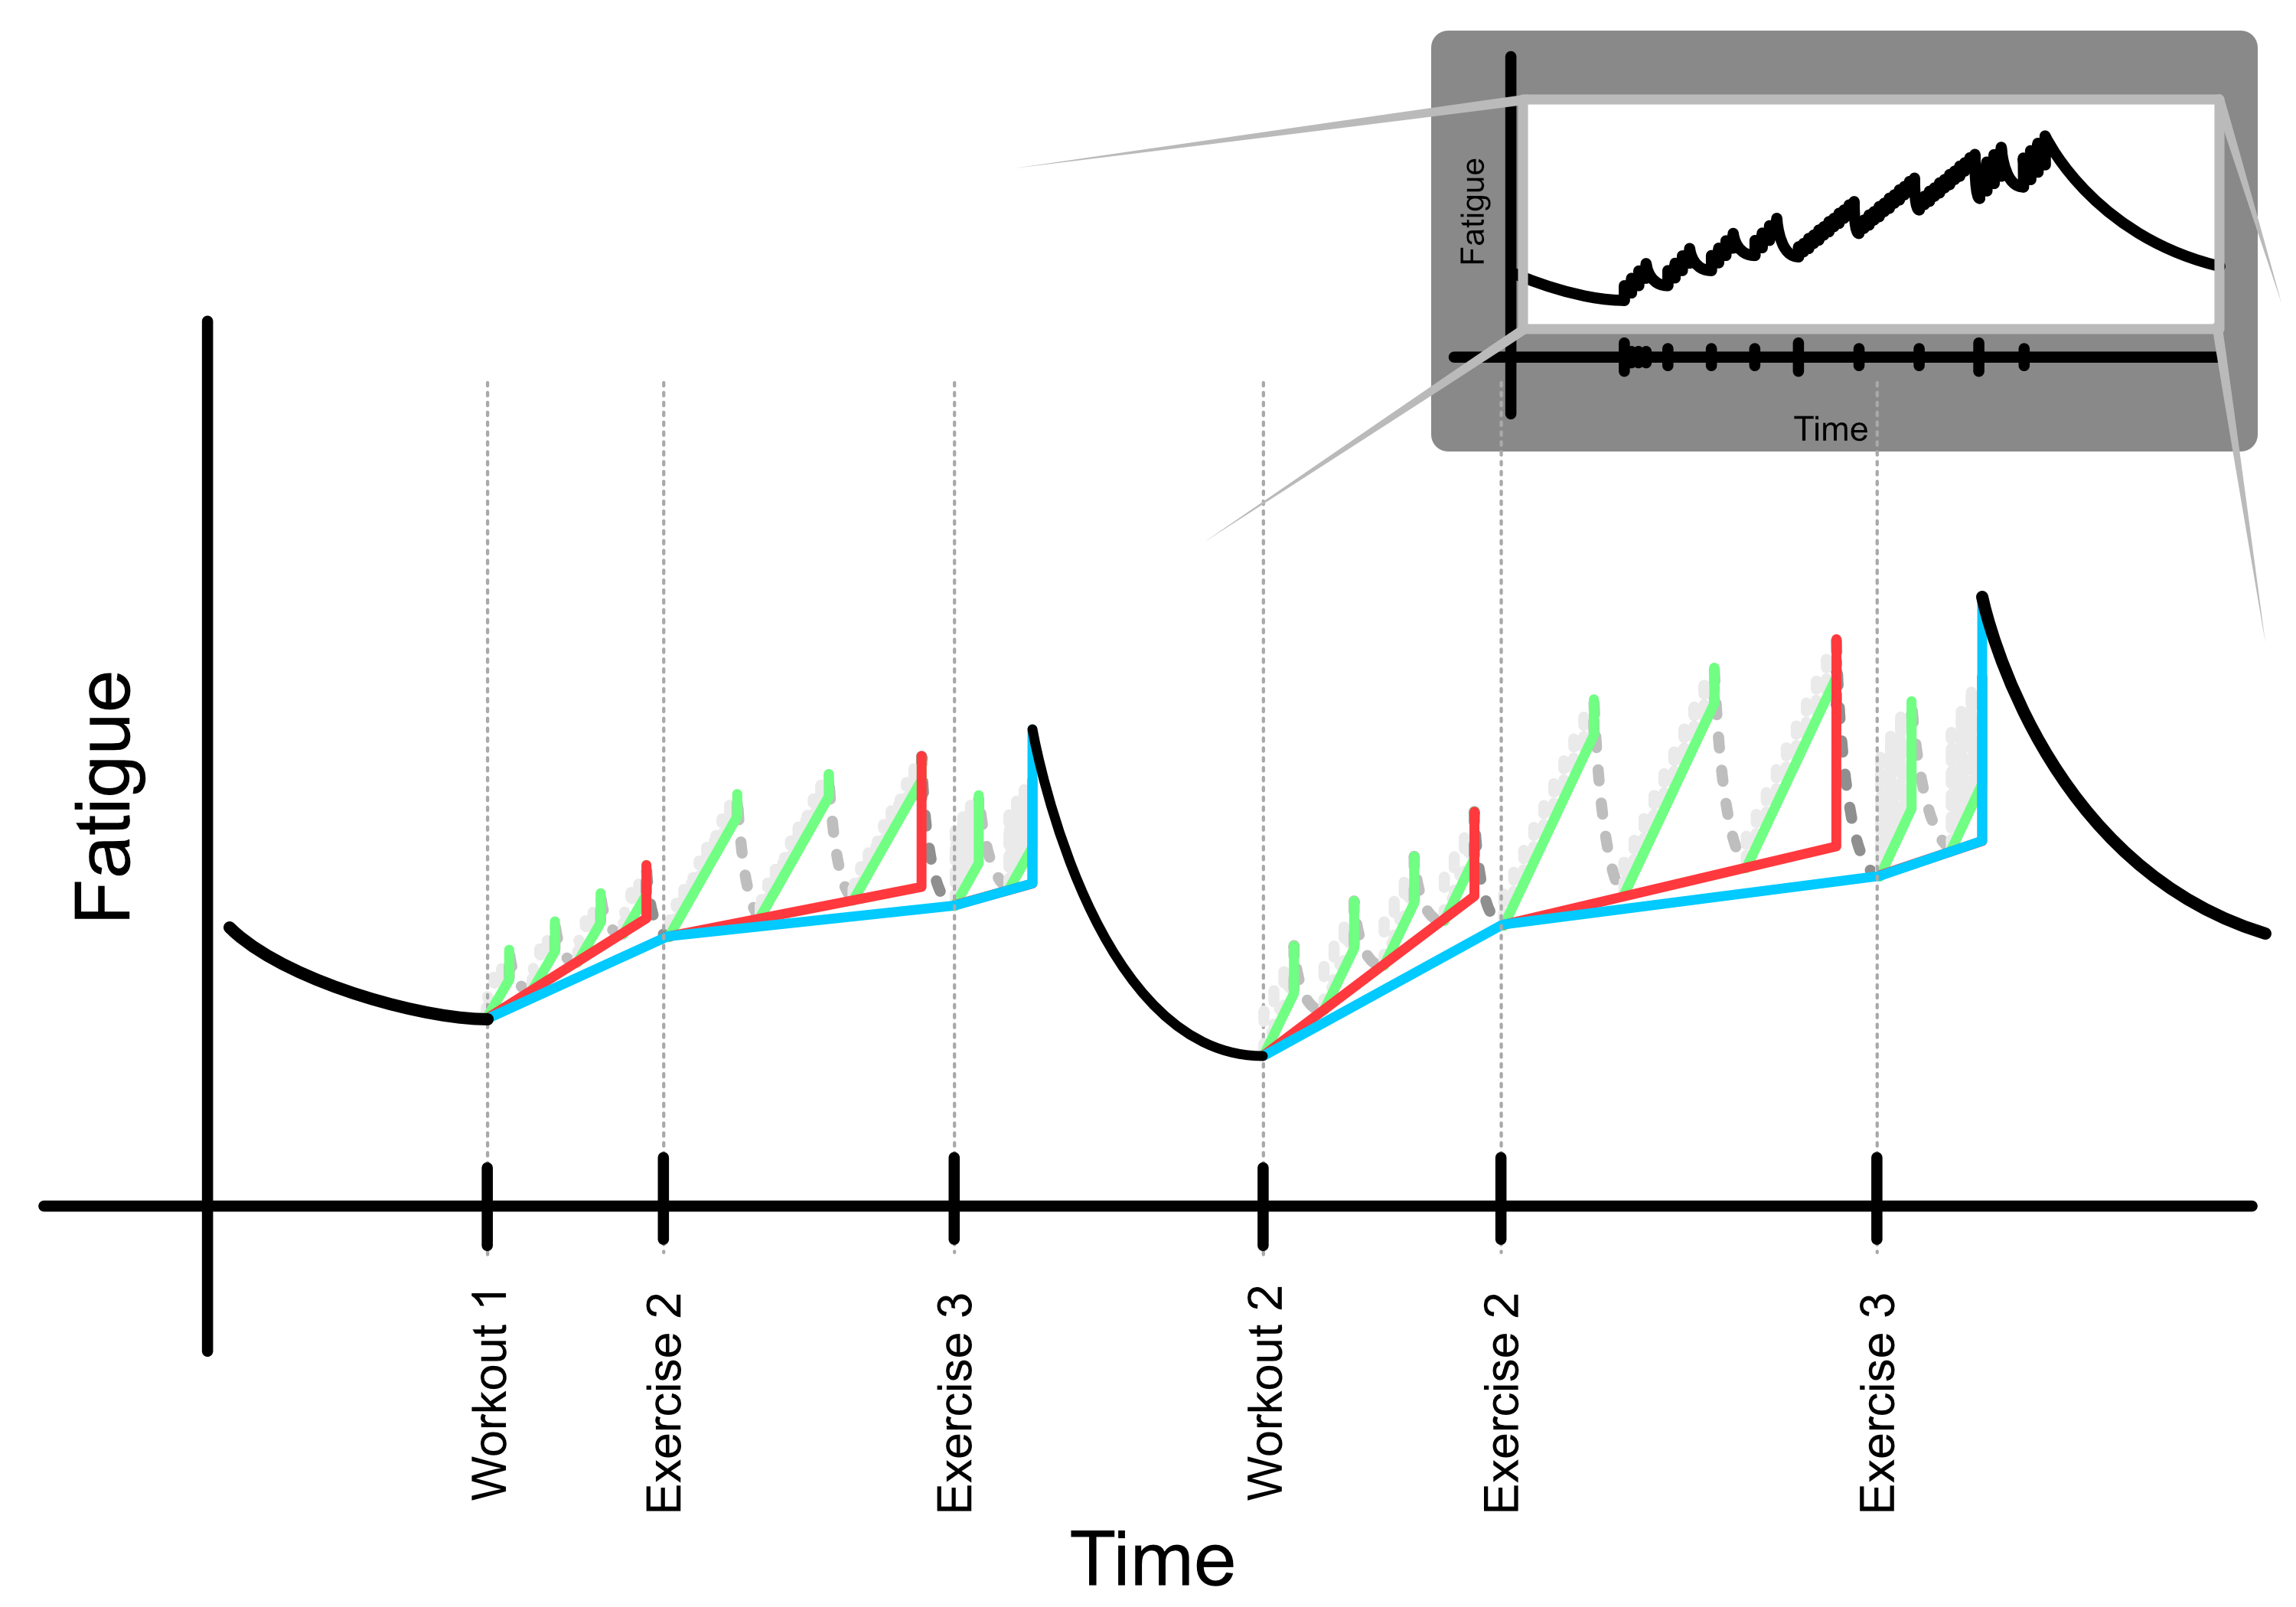
\includegraphics[scale=0.55]{images/p2/ch1/LatentFatigue.png}
    \caption{A figure demonstrating how latent fatigue will accumulate over the course of several workouts.}
    \label{fig:P2C1_LatentFatigue}
\end{figure}

Capturing the latent fatigue from workouts is a very similar process to inter-workout fatigue, the timescale is just a lot larger. As such, a similar equation to what was used in the previous section can be used here. One difference 

\begin{minipage}{\textwidth}
	\begin{equation*}
		F_l =
			F_{w} + 
			\epsilon_2 F_w
			\sum_{i=0}^{n_w-1} \left( 
				s_i r_i E_i^\rho
				\sum_{j=0}^{j=i-1} S(i,j)\left(
					\frac{1}{t_i-t_j+1}
				\right)^\sigma
			\right)
	\end{equation*}
	\centerline{where}
	\begin{equation*}
		\begin{split}
			& n_w \text{ represents the total number of exercises performed} \\
			& S(i,j) \text{ represents a similarity score between exercise }i \text{ and exercise }j \\
			& \rho, \sigma >0
		\end{split}
	\end{equation*}
\end{minipage}\\

\begin{minipage}{\textwidth}
	\begin{equation}
		\label{eq:P2C1_InterWorkoutFatigue}
		\begin{split}
			F_w & = 
			\epsilon_2 F_e 
			\sum_{i=0}^{n_e-1} \left( 
				s_i r_i E_i^\mu 
				\sum_{j=0}^{j=i-1} S(i,j)(n_e-j)^\eta
			\right)
			+ F_e
			\\
			& = \epsilon_6 \left( \frac{E}{10} \right)^\alpha
				\left( \epsilon_5 (r-1)^\beta + 1 \right)
				\left(\epsilon_4 (s-1)^\gamma+1  \right)
				\\
				& \;\;\;
				\left(
					1+\epsilon_3 \sum_{i=0}^{n_e-1} \left( 
						s_i r_i E_i^\mu 
						\sum_{j=0}^{j=i-1} S(i,j)(n_e-j)^\eta
					\right)
				\right)
				\\
				& \;\;\;
				\left(
					1+\epsilon_2 \sum_{i=0}^{n_w-1} \left( 
						s_i r_i E_i^\rho
						\sum_{j=0}^{j=i-1} S(i,j)\left(
							\frac{1}{t_i-t_j+1}
						\right)^\sigma
					\right)
				\right)
			\\
		\end{split}
	\end{equation}
	\centerline{where}
	\begin{equation*}
		\begin{split}
		    & \alpha \ge 1 \\
		    & \beta,\gamma, \mu, \eta, \rho, \sigma > 0 \\
			& 0 \le \epsilon_2, \epsilon_3, \epsilon_4, \epsilon_5, \epsilon_6 \le 1 \\
			& n_e \text{ represents the total number of exercises performed in a workout} \\
			& n_w \text{ represents the total number of exercises performed} \\
			& S(i,j) \text{ represents a similarity score between exercise }i \text{ and exercise }j \\
		\end{split}
	\end{equation*}
\end{minipage}\\

%\begin{minipage}{\textwidth}
%	\begin{equation}
%		\label{eq:P2C1_InterWorkoutFatigue}
%		\begin{split}
%			F_e & = 
%			\epsilon_2 F_w
%			\sum_{i=0}^{n_w-1} \left( 
%				s_i r_i E_i^\rho
%				\sum_{j=0}^{j=i-1} S(i,j)\left(
%					\frac{1}{t_i-t_j+1}
%				\right)^\sigma
%			\right)
%			+F_w
%			\\
%			& =
%			\epsilon_2 \epsilon_3 \epsilon_4 \epsilon_5 \epsilon_6
%			\sum_{i=0}^{n_w-1} \left( 
%				s_i r_i E_i^\rho
%				\sum_{j=0}^{j=i-1} S(i,j)\left(
%					\frac{1}{t_i-t_j+1}
%				\right)^\sigma
%			\right)
%			\sum_{i=0}^{n_e-1} \left( 
%				s_i r_i E_i^\mu 
%				\sum_{j=0}^{j=i-1} S(i,j)(n_e-j)^\eta
%			\right)
%			(s-1)^\gamma 
%			(r-1)^\beta
%			\left(
%				\frac{E}{10} 
%			\right)^\alpha
%			\\
%			& \;\;\; +
%			\epsilon_2 \epsilon_3 \epsilon_4 \epsilon_6
%			\sum_{i=0}^{n_w-1} \left( 
%				s_i r_i E_i^\rho
%				\sum_{j=0}^{j=i-1} S(i,j)\left(
%					\frac{1}{t_i-t_j+1}
%				\right)^\sigma
%			\right)
%			\sum_{i=0}^{n_e-1} \left( 
%				s_i r_i E_i^\mu 
%				\sum_{j=0}^{j=i-1} S(i,j)(n_e-j)^\eta
%			\right)
%			(r-1)^\gamma
%			\left(
%				\frac{E}{10} 
%			\right)^\alpha
%			\\
%			& \;\;\; +
%			\epsilon_2 \epsilon_3 \epsilon_5 \epsilon_6
%			\sum_{i=0}^{n_w-1} \left( 
%				s_i r_i E_i^\rho
%				\sum_{j=0}^{j=i-1} S(i,j)\left(
%					\frac{1}{t_i-t_j+1}
%				\right)^\sigma
%			\right)
%			\sum_{i=0}^{n_e-1} \left( 
%				s_i r_i E_i^\mu 
%				\sum_{j=0}^{j=i-1} S(i,j)(n_e-j)^\eta
%			\right)
%			(r-1)^\beta
%			\left(
%				\frac{E}{10} 
%			\right)^\alpha
%			\\
%			& \;\;\; +
%			\epsilon_2 \epsilon_3 \epsilon_6
%			\sum_{i=0}^{n_w-1} \left( 
%				s_i r_i E_i^\rho
%				\sum_{j=0}^{j=i-1} S(i,j)\left(
%					\frac{1}{t_i-t_j+1}
%				\right)^\sigma
%			\right)
%			\sum_{i=0}^{n_e-1} \left( 
%				s_i r_i E_i^\mu 
%				\sum_{j=0}^{j=i-1} S(i,j)(n_e-j)^\eta
%			\right)
%			\left(
%				\frac{E}{10} 
%			\right)^\alpha
%			\\
%			& \;\;\; +
%			\epsilon_2 \epsilon_4 \epsilon_5 \epsilon_6
%			\sum_{i=0}^{n_w-1} \left( 
%				s_i r_i E_i^\rho
%				\sum_{j=0}^{j=i-1} S(i,j)\left(
%					\frac{1}{t_i-t_j+1}
%				\right)^\sigma
%			\right)
%			(s-1)^\gamma 
%			(r-1)^\beta
%			\left(
%				\frac{E}{10} 
%			\right)^\alpha
%			\\
%			& \;\;\; +
%			\epsilon_2 \epsilon_4 \epsilon_6 
%			\sum_{i=0}^{n_w-1} \left( 
%				s_i r_i E_i^\rho
%				\sum_{j=0}^{j=i-1} S(i,j)\left(
%					\frac{1}{t_i-t_j+1}
%				\right)^\sigma
%			\right)
%			(r-1)^\gamma
%			\left(
%				\frac{E}{10} 
%			\right)^\alpha
%			\\
%			& \;\;\; +
%			\epsilon_2 \epsilon_5 \epsilon_6 
%			\sum_{i=0}^{n_w-1} \left( 
%				s_i r_i E_i^\rho
%				\sum_{j=0}^{j=i-1} S(i,j)\left(
%					\frac{1}{t_i-t_j+1}
%				\right)^\sigma
%			\right)
%			(r-1)^\beta
%			\left(
%				\frac{E}{10} 
%			\right)^\alpha
%			\\
%			& \;\;\; +
%			\epsilon_2 \epsilon_6
%			\sum_{i=0}^{n_w-1} \left( 
%				s_i r_i E_i^\rho
%				\sum_{j=0}^{j=i-1} S(i,j)\left(
%					\frac{1}{t_i-t_j+1}
%				\right)^\sigma
%			\right)
%			\left(
%				\frac{E}{10} 
%			\right)^\alpha
%			\\
%			& \;\;\; +
%			\epsilon_3 \epsilon_4 \epsilon_5 \epsilon_6
%			\sum_{i=0}^{n_e-1} \left( 
%				s_i r_i E_i^\mu 
%				\sum_{j=0}^{j=i-1} S(i,j)(n_e-j)^\eta
%			\right)
%			(s-1)^\gamma 
%			(r-1)^\beta
%			\left(
%				\frac{E}{10} 
%			\right)^\alpha
%			\\
%			& \;\;\; +
%			\epsilon_3 \epsilon_4 \epsilon_6
%			\sum_{i=0}^{n_e-1} \left( 
%				s_i r_i E_i^\mu 
%				\sum_{j=0}^{j=i-1} S(i,j)(n_e-j)^\eta
%			\right)
%			(r-1)^\gamma
%			\left(
%				\frac{E}{10} 
%			\right)^\alpha
%			\\
%			& \;\;\; +
%			\epsilon_3 \epsilon_5 \epsilon_6
%			\sum_{i=0}^{n_e-1} \left( 
%				s_i r_i E_i^\mu 
%				\sum_{j=0}^{j=i-1} S(i,j)(n_e-j)^\eta
%			\right)
%			(r-1)^\beta
%			\left(
%				\frac{E}{10} 
%			\right)^\alpha
%			\\
%			& \;\;\; +
%			\epsilon_3 \epsilon_6
%			\sum_{i=0}^{n_e-1} \left( 
%				s_i r_i E_i^\mu 
%				\sum_{j=0}^{j=i-1} S(i,j)(n_e-j)^\eta
%			\right)
%			\left(
%				\frac{E}{10} 
%			\right)^\alpha
%			\\
%			& \;\;\; +
%			\epsilon_4 \epsilon_5 \epsilon_6
%			(s-1)^\gamma 
%			(r-1)^\beta
%			\left(
%				\frac{E}{10} 
%			\right)^\alpha
%			+
%			\epsilon_4 \epsilon_6 
%			(r-1)^\gamma
%			\left(
%				\frac{E}{10} 
%			\right)^\alpha
%			+
%			\epsilon_5 \epsilon_6 
%			(r-1)^\beta
%			\left(
%				\frac{E}{10} 
%			\right)^\alpha
%			+
%			\epsilon_6
%			\left(
%				\frac{E}{10} 
%			\right)^\alpha
%			\\
%		\end{split}
%	\end{equation}
%	\centerline{where}
%	\begin{equation*}
%		\begin{split}
%		    & \alpha \ge 1 \\
%		    & \beta,\gamma, \mu, \eta, \rho, \sigma > 0 \\
%			& 0 \le \epsilon_2, \epsilon_3, \epsilon_4, \epsilon_5, \epsilon_6 \le 1 \\
%			& n_e \text{ represents the total number of exercises performed in a workout} \\
%			& n_w \text{ represents the total number of exercises performed} \\
%			& S(i,j) \text{ represents a similarity score between exercise }i \text{ and exercise }j \\
%		\end{split}
%	\end{equation*}
% \end{minipage}\\


\section{What is Similarity?}
\label{sec:P2C1_WhatIsSimilarity}

There has been discussion about exercise similarity, but there has been no discussion about what constitutes similarity. Before continuing the details of what makes exercises similar needs to be established.






\section{Summary}

This chapter outlined a model that will be fully realized in the remaining chapters of part 1. Doing this will create surfaces that will need to be fitted to the data. These surfaces will be called \textit{potential surfaces}, because they represent a lifters potential performance. It is important to conceptualize that every combination of sets, reps, weight, and effort defined by a potential surface is theoretically possible for a lifter to complete. This is the foundation this entire book will build off of.

Finally, the approximate form of the effort-fatigue model can be defined, and is shown in equation \ref{eq:PotentialSurfaceEquation}. Again, this may seem like a finished equation, but remember this is just a template. The surfaces in the next several chapters will create final equations to concretely realize the ideas of the effort-fatigue model. These equations may take very different forms, but the principles of the effort-fatigue model will still stand behind them.

\begin{equation}
	\label{eq:PotentialSurfaceEquation}
	\begin{split}
		I & \hat{=} E_{tot} \hat{-} F_{tot} \\
		I & \hat{=} \epsilon_1 E \hat{-} 
			\left(
				\epsilon_6 \left( \frac{E}{10} \right)^\alpha
				\left( \epsilon_5 (r-1)^\beta + 1 \right)
				\left( \epsilon_4 (s-1)^\gamma+1 \right)
				\right.
				\\
				& \;\;\;\;\;\;\;\;\;\;\;\;\;\;
				\left(
					1+\epsilon_3 \sum_{i=0}^{n_e-1} \left( 
						s_i r_i E_i^\mu 
						\sum_{j=0}^{j=i-1} S(i,j)(n_e-j)^\eta
					\right)
				\right)
				\\
				& \;\;\;\;\;\;\;\;\;\;\;\;\;\;
				\left.
				\left(
					1+\epsilon_2 \sum_{i=0}^{n_w-1} \left( 
						s_i r_i E_i^\rho
						\sum_{j=0}^{j=i-1} S(i,j)\left(
							\frac{1}{t_i-t_j+1}
						\right)^\sigma
					\right)
				\right)
			\right)
	\end{split}
\end{equation}







%\section{Augmenting The Data: Improvising for What Can't Be Measured}
%\label{sec:AugmentedDataSet}
%
%Some readers may have noticed the lack of data that records fatigue. This is a direct result of not being able to measure fatigue in a timely manner that is also unobtrusive to training. Many of the tests used to measure fatigue require tools or extensive time that is simply not conducive to a training environment, especially when it comes to short term fatigue measurements such as inter-set fatigue. However, fatigue is a large factor that determines what a lifter can do. While fatigue cannot be directly represented due to it not being part of the data, it effects are still visible. Things like sets that took more effort than they should have can be attributed to fatigue. Any modeling done will need a way to determine what affects fatigue had. To help accomplish this, the data set will be augmented with \textit{indexes} that provide measurements similar to how fatigue would be present if it were measured directly. This may seem strange, so hopefully the first example will help clear things up.
%
%Consider inter-workout fatigue. Every rep of every exercise a lifter does will increase the lifters inter-workout fatigue. To represent this, an inter-workout fatigue index will be added to the data set. To calculate the inter-workout fatigue index, the total number of reps completed across all exercises before the current exercise will be summed together. The arithmetic sequence shown in equation \ref{eq:InterWorkoutFatigueEquation} demonstrates this, and can be used when adding an exercise to a workout. Note how the first inter-workout fatigue index is $0$. This reflects the lifter not having generated any inter-workout fatigue when first starting a workout. Every value after that then reflects the inter-workout fatigue that was present \textit{before} each exercise was done. Only measuring the fatigue that was present before the exercise was performed is important because it represents the fatigue the exercise was performed with, ignoring the fatigue that will be generated while doing the exercise. This is consistent with how any real measurements of fatigue would be recorded.
%
%\begin{equation}
%	\label{eq:InterWorkoutFatigueEquation}
%	\begin{split}
%		F_{w,i} & = 
%		\begin{cases}
%			s_{i-1}r_{i-1}+F_{w,i-1} \;\; & \text{if }t_i=t_{i-1} \\
%			0 \;\; & \text{otherwise}
%		\end{cases}
%		\\
%		F_{w,0} & = 0
%	\end{split}
%\end{equation}
%
%By defining the inter-workout fatigue index this way, it will increase when a direct measurement of inter-workout fatigue would. Having the index value increase as fatigue increases and decrease as fatigue decreases is the key to making this strategy work, as any modeling later will be able to scale the results as needed through constants. \footnote{This method does assume fatigue increases with reps linearly. An argument could be made for greater than linear increases in fatigue, but for simplicities sake it will be assumed to increase linearly. Note that if further research proves a non-linear relationship the index values could easily be adjusted to follow the correct non-linear pattern. This could also be adjusted for directly in the model if necessary.} Table \ref{tab:IndexesExample} shows an example of the inter-workout fatigue index along with how it's values were calculated above it. \footnote{Note how the last value is not shown in data set because it is past the end of the workout.}
%
%\begin{equation*}
%	\begin{aligned}
%		F_{w,0} & =0 \\
%		F_{w,1} & =1(1)+0=1 \\
%		F_{w,2} & =5(4)+1=21 \\
%		F_{w,3} & =1(10)+21=31 \\
%		F_{w,4} & =5(5)+31=56 \\
%		F_{w,5} & =3(12)+56=92  \\
%	\end{aligned}
%\end{equation*}
%
%\begin{table}[h]
%	\centering
%	\begin{tabular}{c|c|c|c|c|c|c|c}
%		Date & Exercise & Sets & Reps & Weight & Effort & $F_w$ Index & $F_e$ Index \\
%        \hline
%        Mon, July 4\textsuperscript{th} & Deadlifts & $1$ & $1$ & $455$ lbs & $8.5$ & $0$ & $0$ \\
%        Mon, July 4\textsuperscript{th} & Deadlifts & $5$ & $4$ & $405$ lbs & $8.5$ & $1$ & $1$ \\
%        Mon, July 4\textsuperscript{th} & Deadlifts & $1$ & $10$ & $315$ lbs & $7$ & $21$ & $21$ \\
%        Mon, July 4\textsuperscript{th} & Barbell Rows & $5$ & $5$ & $225$ lbs & $6.5$ & $31$ & $0$ \\
%        Mon, July 4\textsuperscript{th} & Hyperextensions & $3$ & $12$ & $45$ lbs & $-$ & $56$ & $0$ \\
%        Tue, July 5\textsuperscript{th} & SSB Squats & $5$ & $8$ & $255$ lbs & $6$ & $0$ & $0$ \\
%        \dots & \dots & \dots & \dots & \dots & \dots & \dots & \dots \\
%	\end{tabular}
%	\caption{A table demonstrating the way various fatigue index values are calculated. Note how $F_w$ increases with the total number of reps. $F_e$ increases with the number times a lift was performed, also in accordance to the total number of reps. $F_w$ resets to $0$ on the new workout and $F_e$ resets to $0$ on each different exercise.}
%	\label{tab:IndexesExample}
%\end{table}
%
%Inter-exercise fatigue can have the same index scheme but instead of incrementing over the entire workout, it only increments according to sets of the same exercise, resetting each time a new exercise is started. Equation \ref{eq:InterExerciseFatigueEquation} can be used to calculate the inter-exercise fatigue index. Note that this equation is only valid within the context of a single exercise. Table \ref{tab:IndexesExample} also shows an example of inter-exercise fatigue.
%
%% TODO - change  t_i to exercise_i
%\begin{equation}
%	\label{eq:InterExerciseFatigueEquation}
%	\begin{split}
%		F_{e,i} & =
%		\begin{cases}
%			s_{i-1}r_{i-1}+F_{e,i-1} \;\; & \text{if }E_{x,i}=E_{x,i-1} \\
%			0 \;\; & \text{otherwise}
%		\end{cases}
%		\\
%		F_{e,0} & = 0
%	\end{split}
%\end{equation}
%
%The last two categories of fatigue are inter-set fatigue and latent fatigue. It is tempting to add an index for inter-set fatigue, but the set and reps values already serve this purpose. Latent fatigue's behavior is not so cut and dry as the other types of fatigue. It can fluctuate based on many factors, many of which are entirely independent from the gym. This makes it difficult to make an index value for latent fatigue as the key to making any index work is to make it increase and decrease as the original measurement would. If those increases and decreases cannot be accurately predicted and represented then an index cannot be used reliably. While the factors outside the gym cannot be controlled for due to the lack of data representing them, the factors that are present from the gym can, and should, be considered. Doing this however will require it's own chapter, chapter \ref{sec:}.
